\documentclass[russian,14pt]{eskdtext}
\usepackage[numbertop, numbercenter]{eskdplain}
\usepackage[utf8x]{inputenc}

\usepackage{setspace}
\onehalfspacing % полуторный интервал для всего текста

% - Подключаем шрифты из пакета scalable-cyrfonts-tex
\usepackage{cyrtimes}

% - Отступ красной строки
\setlength{\parindent}{1.25cm}

% - Убирает точку в списке литературы
\makeatletter
\def\@biblabel#1{#1 }

% ограничение для оглавления
%\usepackage{tocvsec2}
\setcounter{tocdepth}{2}

% - Точки для всех пунктов в оглавлении
\renewcommand*{\l@section}{\@dottedtocline{1}{1.5em}{2.3em}}
\renewcommand*{\l@subsection}{\@dottedtocline{1}{1.5em}{2.3em}}
%\renewcommand*{\l@subsubsection}{\@dottedtocline{1}{1.5em}{2.3em}}

% - Для переопределения списков
\renewcommand{\theenumi}{\arabic{enumi}}
\renewcommand{\labelenumi}{\theenumi)}
\makeatother

\usepackage{enumitem}
\setlist{nolistsep, itemsep=0.3cm,parsep=0pt}

% - ГОСТ списка литературы
\bibliographystyle{gost71u2003}

% - Верикальные отступы заголовков 
\ESKDsectSkip{section}{1em}{1em}
\ESKDsectSkip{subsection}{1em}{1em}
\ESKDsectSkip{subsubsection}{1em}{1em}

% - Изменение заголовков
\usepackage{titlesec}
\titleformat{\section}{\normalfont\normalsize\centering}{\thesection}{1.0em}{}
\titleformat{\subsection}{\normalfont\normalsize\centering}{\thesubsection}{1.0em}{}
\titleformat{\subsubsection}{\normalfont\normalsize\centering}{\thesubsubsection}{1.0em}{}
\titleformat{\paragraph}{\normalfont\normalsize\centering}{\theparagraph}{1.0em}{}

% - Оставим место под ТЗ 
%\setcounter{page}{4}

% - Для больших таблиц
\usepackage{longtable}
\usepackage{tabularx}
\renewcommand{\thetable}{\thesection.\arabic{table}}

% - Используем графику в документе
\usepackage{graphicx}
\graphicspath{{images/}}
\renewcommand{\thefigure}{\thesection.\arabic{figure}}

% - Счётчики
\usepackage{eskdtotal}

% - Выравнивание по ширине
\sloppy

% - Разрешить перенос двух последних букв слова
\righthyphenmin=2

% - Оформление списков
\RequirePackage{enumitem}
\renewcommand{\alph}[1]{\asbuk{#1}}
\setlist{nolistsep}
\setitemize[1]{label=--, fullwidth, itemindent=\parindent, 
  listparindent=\parindent}% для дефисного списка
\setitemize[2]{label=--, fullwidth, itemindent=\parindent, 
  listparindent=\parindent, leftmargin=\parindent}
\setenumerate[1]{label=\arabic*), fullwidth, itemindent=\parindent, 
  listparindent=\parindent}% для нумерованного списка
\setenumerate[2]{label=\alph*), fullwidth, itemindent=\parindent, 
  listparindent=\parindent, leftmargin=\parindent}% для списка 2-ой ступени, который будет нумероваться а), б) и т.д.
  
% - Оформляем листинг кода (не использовать комментарии на русском!)
\usepackage{listings}  
\lstset{basicstyle=\ttfamily\scriptsize}
\lstset{extendedchars=\true}

% - выводим текст как есть с размером шрифта scriptsize
\makeatletter
\def\verbatim{\scriptsize\@verbatim \frenchspacing\@vobeyspaces \@xverbatim}
\makeatother

% - Вставка pdf
\usepackage{pdfpages}

%межстрочный интервал
\usepackage{setspace}
\linespread{1.5}

\begin{document}
 \newpage
\ESKDthisStyle{empty}

\begin{center}
Министерство образования и науки Российской Федерации\\
Федеральное государственное бюджетное образовательное учреждение высшего профессионального образования\\
ТОМСКИЙ ГОСУДАРСТВЕННЫЙ УНИВЕРСИТЕТ СИСТЕМ УПРАВЛЕНИЯ И РАДИОЭЛЕКТРОНИКИ (ТУСУР)\\
Кафедра комплексной информационной безопасности электронно-вычислительных систем (КИБЭВС)\\
\end{center}

\vspace{2cm}

\begin{center}
Отчет по преддипломной практике \\
на тему \\
``Выбор протокола взаимодействия между датчиками и центральным сервером АСКУЭ''
\end{center}

\vspace{2cm}

\begin{flushright}
Выполнил: \\
студент гр. 720-1 \\
\underline{\hspace{2.5cm}}Д.С. Никифоров \\
"\underline{\hspace{1cm}}"\underline{\hspace{3cm}} 2015г.\\
\end{flushright}

\begin{flushright}
Утвердил: \\
Доцент каф.КИБЭВС \\
\underline{\hspace{2.5cm}}А.А. Конев \\
"\underline{\hspace{1cm}}"\underline{\hspace{3cm}} 2015г.\\
\end{flushright}

\vfill
\begin{center}
Томск -- 2015
\end{center}
 \newpage
\ESKDthisStyle{empty}
\paragraph*{\hfill РЕФЕРАТ \hfill}
Отчет по преддипломной практике содержит \ESKDtotal{page} страниц, \ESKDtotal{figure} рисунков,  6 таблиц, 3 источника.

АСКУЭ, ПРОТОКОЛ, СВЯЗЬ, СЕРВЕР, TCP/IP, QT, СЕТЬ, SQLITE.

Цель работы -- создание протокола взаимодействия между сервером и устройствами сбора данных АСКУЭ.

В ходе работы был сделан обзор существующих протоколов; реализована программа, эмулирующая функцию приема/передачи данных УСПД; реализована программа, осуществляющая взаимодействие с эмулятором и сохраняющая данный от эмулятора в базу данных.

Пояснительная записка выполнена при помощи системы компьютерной вёрстки \LaTeX.
 \newpage
\ESKDthisStyle{empty}

\begin{center}
Министерство образования и науки Российской Федерации\\
Федеральное государственное бюджетное образовательное учреждение высшего профессионального образования\\
ТОМСКИЙ ГОСУДАРСТВЕННЫЙ УНИВЕРСИТЕТ СИСТЕМ УПРАВЛЕНИЯ И РАДИОЭЛЕКТРОНИКИ (ТУСУР)\\
Кафедра комплексной информационной безопасности электронно-вычислительных систем (КИБЭВС)\\
\end{center}

\begin{flushright}
 \begin{minipage}{0.4\textwidth}
  УТВЕРЖДАЮ \\
  Зав. кафедры КИБЭВС \\
  \underline{\hspace{2.5cm}}А.А. Шелупанов \\
  "\underline{\hspace{1cm}}"\underline{\hspace{3cm}} 2015г.
 \end{minipage}
\end{flushright}

\vspace{2cm}

\begin{center}
 ЗАДАНИЕ \\
% На преддипломную практику
\end{center}

Студенту Дмитрию Сергеевичу Никифорову группы 720-1, факультета безопасности.

% 1. Тема преддипломной практики: ``Механизм взаимодействия датчиков и центрального сервера АСКУЭ''
% 
% 2. Исходные данные к проекту: Документация к проекту разработки АСКУЭ.
% 
% Руководитель практики: \\ директор ЦСП ТУСУР Антон Александрович Конев. 
% 
% \hfill Подпись руководителя: \underline{\hspace{2.5cm}}
% 
% \hfill "\underline{\hspace{1cm}}"\underline{\hspace{3cm}} 2015г.
% 
% Задание принял к исполнению
% 
% Студент гр. 720-1 Дмитрий Сергеевич Никифоров \hfill \underline{\hspace{2.5cm}}
% 
% \hfill "\underline{\hspace{1cm}}"\underline{\hspace{3cm}} 2015г. %TODO переделать задание
 \newpage
 \tableofcontents
 \newpage
\section{Введение}
\setcounter{figure}{0}

%Целью данной работы является определить наиболее популярные протоколы передачи данных, поддерживаемые в приборах и системах учета, с целью их анализа, выбора и дальнейшей реализации в разрабатываемой автоматизированной системе коммерческого учета энергоресурсов, 

Целью данной работы является создание протокола взаимодействия между сервером сбора данных (ССД) и устройствами съема и передачи данных(УСПД) в автоматизированной системе коммерческого учета энергоресурсов (АСКУЭ).

Создание нового протокола необходимо для использования АСКУЭ в сфере ЖКУ, так как существующие протоколы ориентированы на использования в пределах предпприятий, из-за чего существующие протоколы не учитывают аспекты информационной безопасности, в протоколах отсуствует авторизация, линии связи обладают недостаточно дальностью передачи сигнала без использования повторителей. 

Всё это приводит к серьезным проблемам при использвании АСКУЭ в условиях ЖКУ. Появляется проблема передачи данных от УСПД до ССД, так как для использования существующих протоколов необходимо прокладывать линии связи. Использование протоколов так же не гарантиреут подлиности и аутентичность передаваемых данных. 

%После чего необходимо реализовать функции взаимодействия сервера с устройством съема и передачи данных (УСПД) по данному протоколу, в том числе разработать систему команд взаимодействия с УСПД.
 \newpage
\section{Описание разрабатываемой автоматизированной системы коммерческого учета энергоресурсов}
\setcounter{figure}{0}

Основными  потребителями  электросчетчиков российского производства являются страны СНГ, Украина и Казахстан – лидеры по потреблению в 2007-2013 году (на долю экспорта в эти страны приходится около  80\% [1] ). Для учета использования электроэнергии существуют автоматизированные системы коммерческого учета электроэнергии (АСКУЭ).

Автоматизированная система коммерческого учета энергоресурсов (АСКУЭ) - это программно-аппаратный комплекс, предназначенный для сбора, хранени и обработки инофрмации о потреблении энергоресурсов на объекте. 

Аппаратная часть представлена устройствами учета(УУ), устройствами сбора и передачи данных(УСПД), а так же центральным сервером(ЦС).

Программная часть включает в себя прошивки УУ и УСПД, ПО для ЦС.

ПО ЦС предназначено для сбора показаний с точек учета энергоресурсов, а также архивирования, хранения, анализа и визуализации полученных данных, формирования отчетов. Под показаниями подразумеваются данные о потребляемой мощности электроэнергии потребителями однофазных и трехфазных сетей.

Областью применения ПО ЦС являются объекты жилого, коммерческого и производственного назначения.

ПО ЦС — это программный комплекс, который должен включать в себя сервер баз данных, сервер сбора данных(ССД), сервер приложений, web-сервер, АРМ оператора, АРМ администратора, АРМ клиента, АРМ сервисного инженера(АРМ СИ).

ПО ССД должно выполнять следующие функции:
\begin{itemize}
 \item взаимодействие с УСПД и счетчиками (опрос и сбор данных);
 \item взаимодействие с СБД (запись обработанных данных для дальнейшей работы с ними);
 \item преобразование полученных данных в удобный для дальнейшей обработки формат;
 \item мониторинг и обработка ошибок;
 \item журналирование событий ССД.
\end{itemize}

ПО ЦС представляет собой иерархическую систему сбора, передачи и хранения данных (рис. \ref{irsh:irsh}). Информация от первичных приборов учета посредством УСПД поступает на ССД, который обеспечивает ее обработку и запись на СБД.

\begin{figure}[h!]
 \center{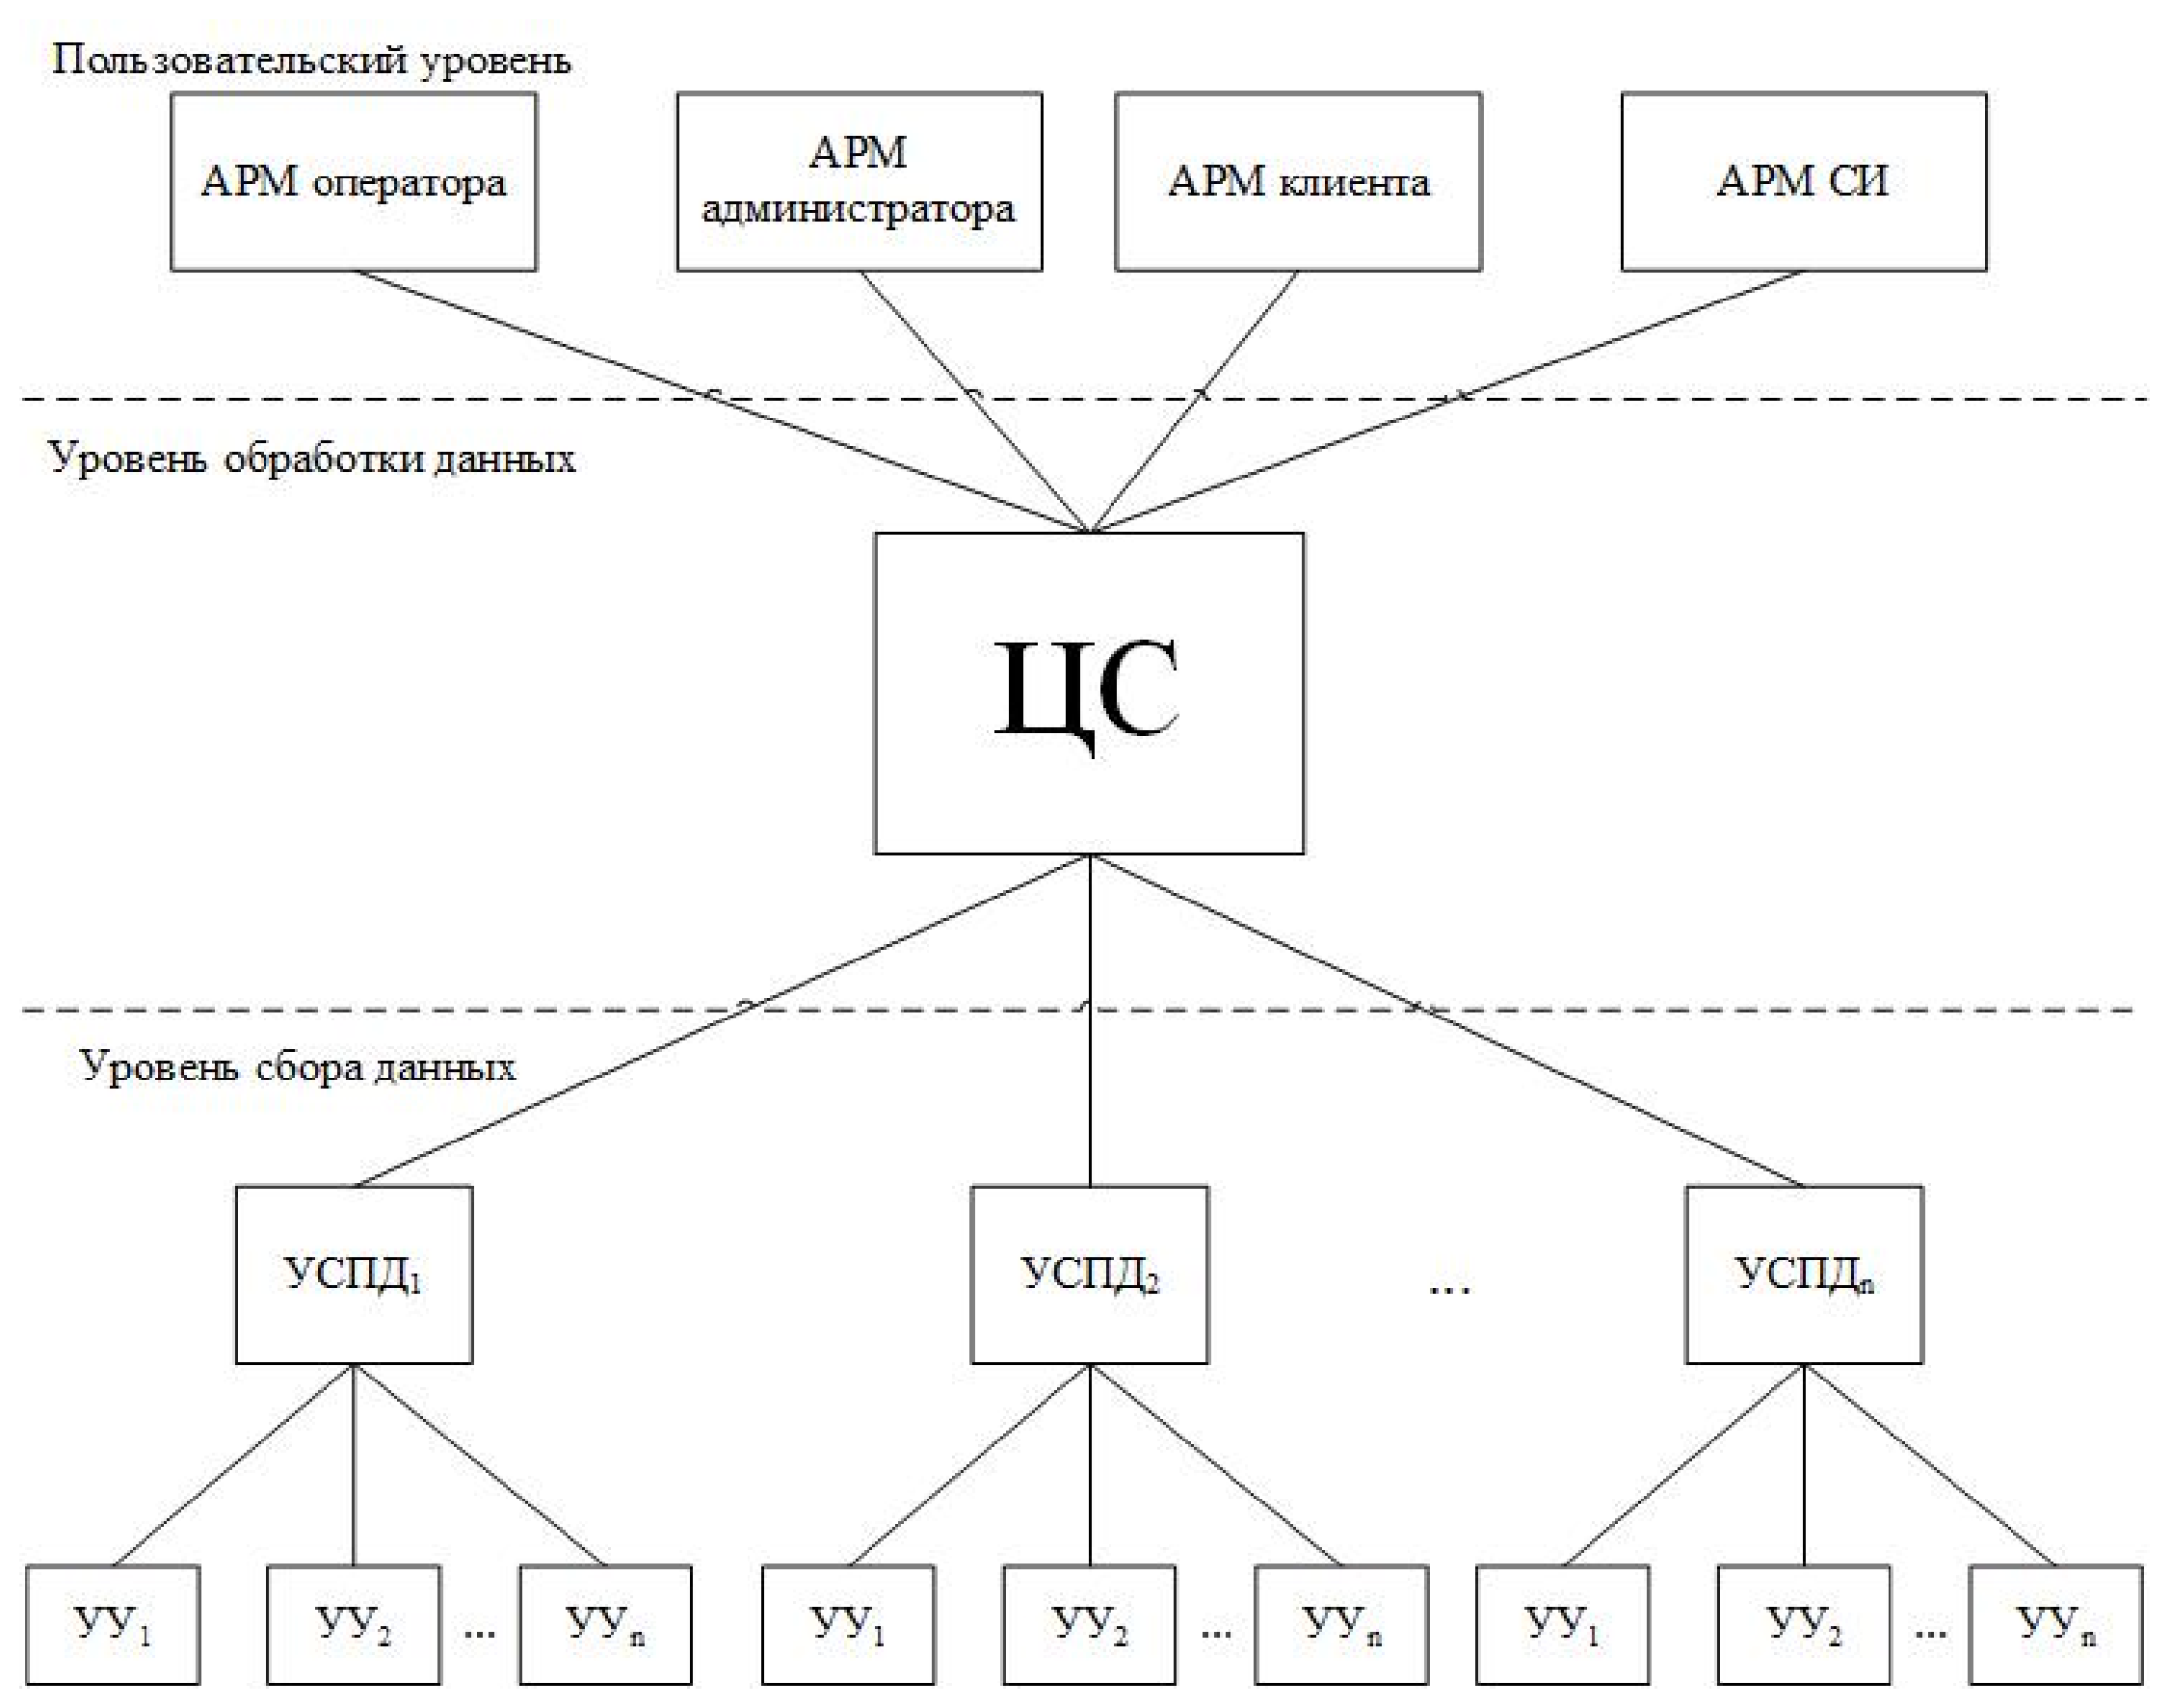
\includegraphics[width=0.8\linewidth]{irsh}}
 \caption{Структурная схема АСКУЭ}
 \label{irsh:irsh}
\end{figure}

\subsection{Описание сервера сбора данных}

ССД обслуживает низкоуровневое взаимодействие с УСПД. После получения данных этот блок передает информацию модульной системе драйверов. Система драйверов осуществляет взаимодействие на верхнем уровне модели OSI. За счет модульности обеспечивается расширение парка поддерживаемого оборудования. Также ССД содержит систему управления сетью и взаимодействия с базой данных: он осуществляет контроль работоспособности сети, выполняет отбраковку данных, отвечает за принятие решений о повторном запросе на сбор данных, классифицирует информацию, обеспечивает контроль единого времени и осуществляет запись информации в базу данных.

Логически ПО ССД можно разделить на 3 блока, каждый из которых выполняет отдельную задачу:
\begin{enumerate}
\item блок контроля приема и передачи данных, который отвечает за взаимодействие ССД с УСПД;
\item временная база данных (ВБД). В ходе проектирования ПО ССД было рассмотрено два варианта обработки и записи данных с УСПД/УУ на СБД: 
\begin{itemize}
\item обработка и запись данных на СБД по мере их поступления от УСПД;
\item запись поступающих данных в ВБД и последующая обработка и передача на СБД.
\end{itemize}
\item блок обработки данных.
\end{enumerate}

Использование первого варианта может привести к потере данных, так как вновь поступающие данные не будут успевать обрабатываться ПО ССД. Второй вариант позволяет обеспечить целостность поступивших данных, поэтому он является более предпочтительным.

Обобщенная функциональная схема функционирования ПО ССД представлена на рисунке \ref{fs_ssd:fs_ssd}.

\begin{figure}[h!]
 \center{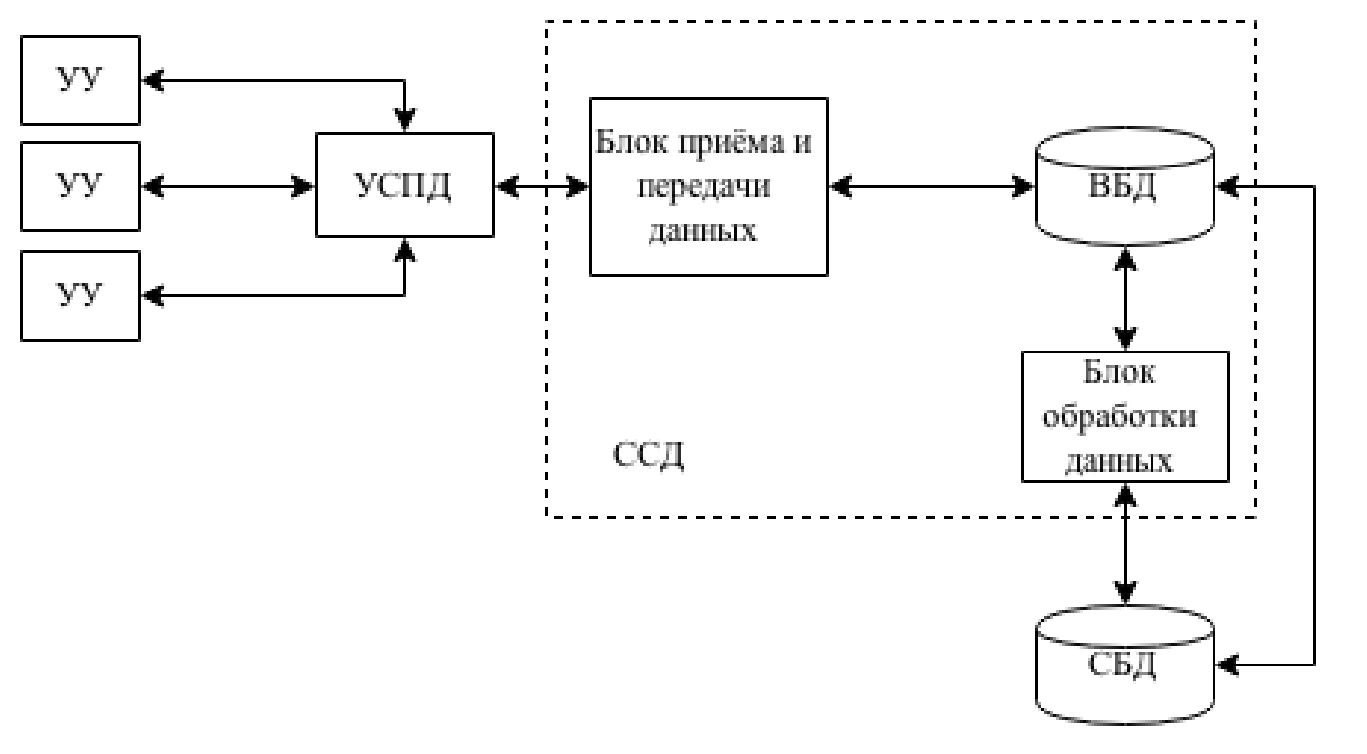
\includegraphics[width=0.8\linewidth]{fs_ssd}}
 \caption{Функциональная схема ССД}
 \label{fs_ssd:fs_ssd}
\end{figure}

Сервер сбора данных должен отвечать следующим требованиям:

\begin{itemize}
 \item работать с УСПД в количестве до 10000 устройств;
 \item передавать данные по сети интернет;
 \item контроль подключаемых устройств;
 \item контроль целостности данных;
 \item возможность добавления УСПД в запущенную систему;
 \item оперативная реакция на сигналу УСПД о неполадках.
\end{itemize}

\subsection{Описание устройства сбора и передачи данных}%TODO

Устройство сбора и передачи данных является промежуточным звеном между устройствами учета и сервером сбора данных. Оно предназначено для непосредственного управления устройствами учета, их опроса, настройки и диагностики. Всю информацию от устройств учета и о их состоянии ССД получает от УСПД.

Требования, предъявляемые к УСПД:

\begin{itemize}
 \item контроль подключений;
 \item идентификация и аутентификация пользователей;
\end{itemize}

\subsection{Взаимодействие ССД и УСПД}

Сервер сбора данных должен запрашивать с УСПД показагия всех УУ и информацию о состоянии УУ и самого УСПД. Связь устанавливается при запросе данных. Обмен данных должен начинаться с идентификации и аутентификации ССД на УСПД. После окончания сбора данных производится завершение сеанса на УСПД и разрыв соединения.

Функциональная схема данного процеса представлена на рисунке \ref{img:main_idef0}.

\begin{figure}[!Ht]
 \center{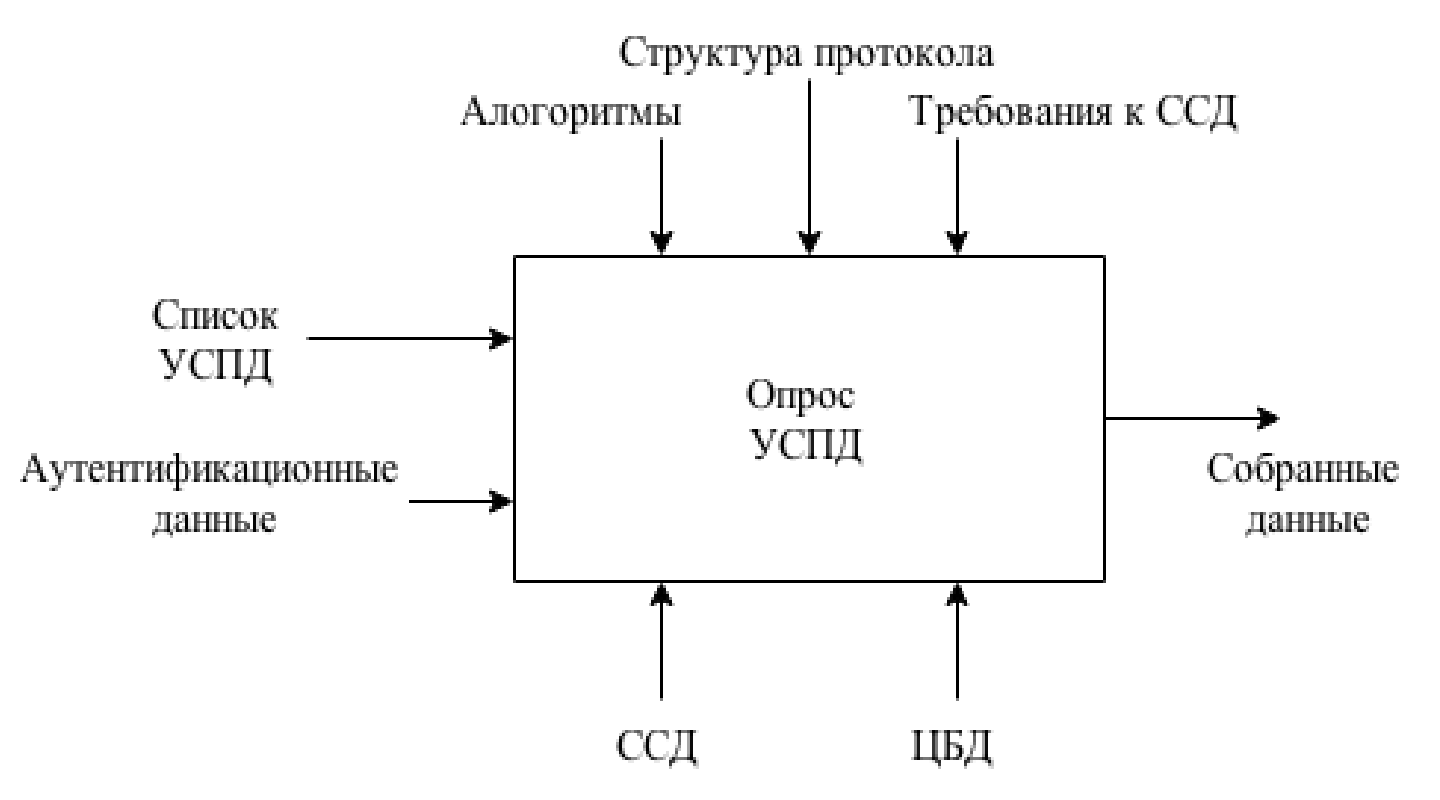
\includegraphics[width=0.8\linewidth]{main_idef0}}
 \caption{Функциональная схема процесса опроса УСПД}
 \label{img:main_idef0}
\end{figure}

После получения данных со всех УСПД происходит их обработка и отравка в центральнуб базу данных(ЦБД). В ЦБД так же хранится список всех УСПД, подконтрольных ССД.

Данные необходимо шифровать при передаче.

В разрабатываемой системе сервер является инициатором всех обменов данными, а клиенты ожидают запроса для передачи данных. Схема взаимодействия приведена на рисунке \ref{scheme2:scheme2}.

\begin{figure}[!ht]
 \center{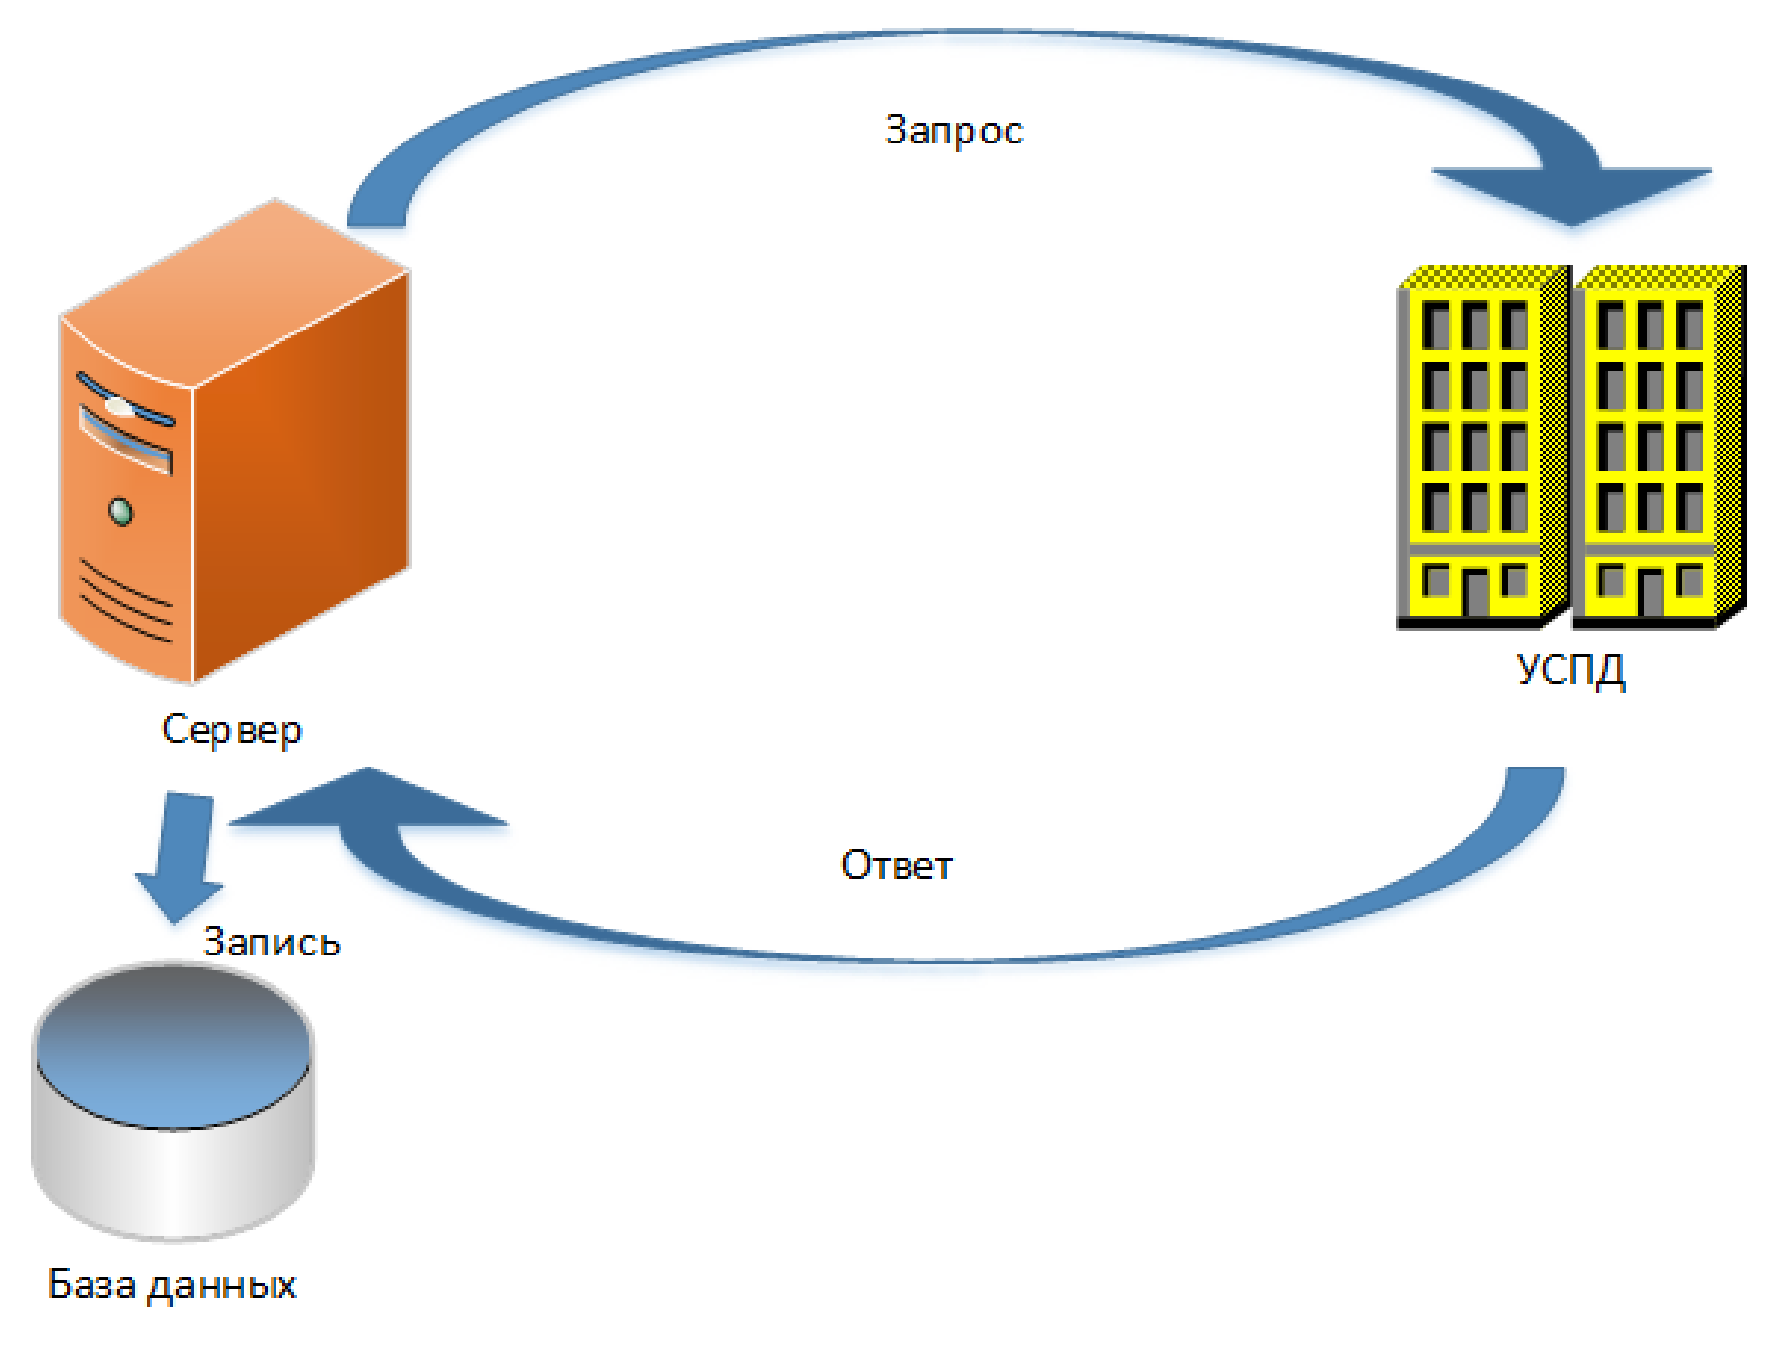
\includegraphics[width=0.8\linewidth]{scheme2}}
 \caption{Схема взаимодействия сервера с УСПД}
 \label{scheme2:scheme2}
\end{figure}

Данный механиз позволяет реализовать опрос УСПД по списку, хранящемуся на сервере, что исключит возможность отправки данных с несанкционированных устройств. Так же появляется возможность обнаружения неисправности УСПД либо ошибки сети, на который сервер будет реагировать предупреждениями. 

Данные, полученные с УСПД, записываются во временную базу данных для последующей обработки и отправки на центральный сервер. В этой же базе данных хранится список всех УСПД, подконтрольных данному серверу. Схема представлена на рисунке \ref{scheme3:scheme3}.

\begin{figure}[!ht]
 \center{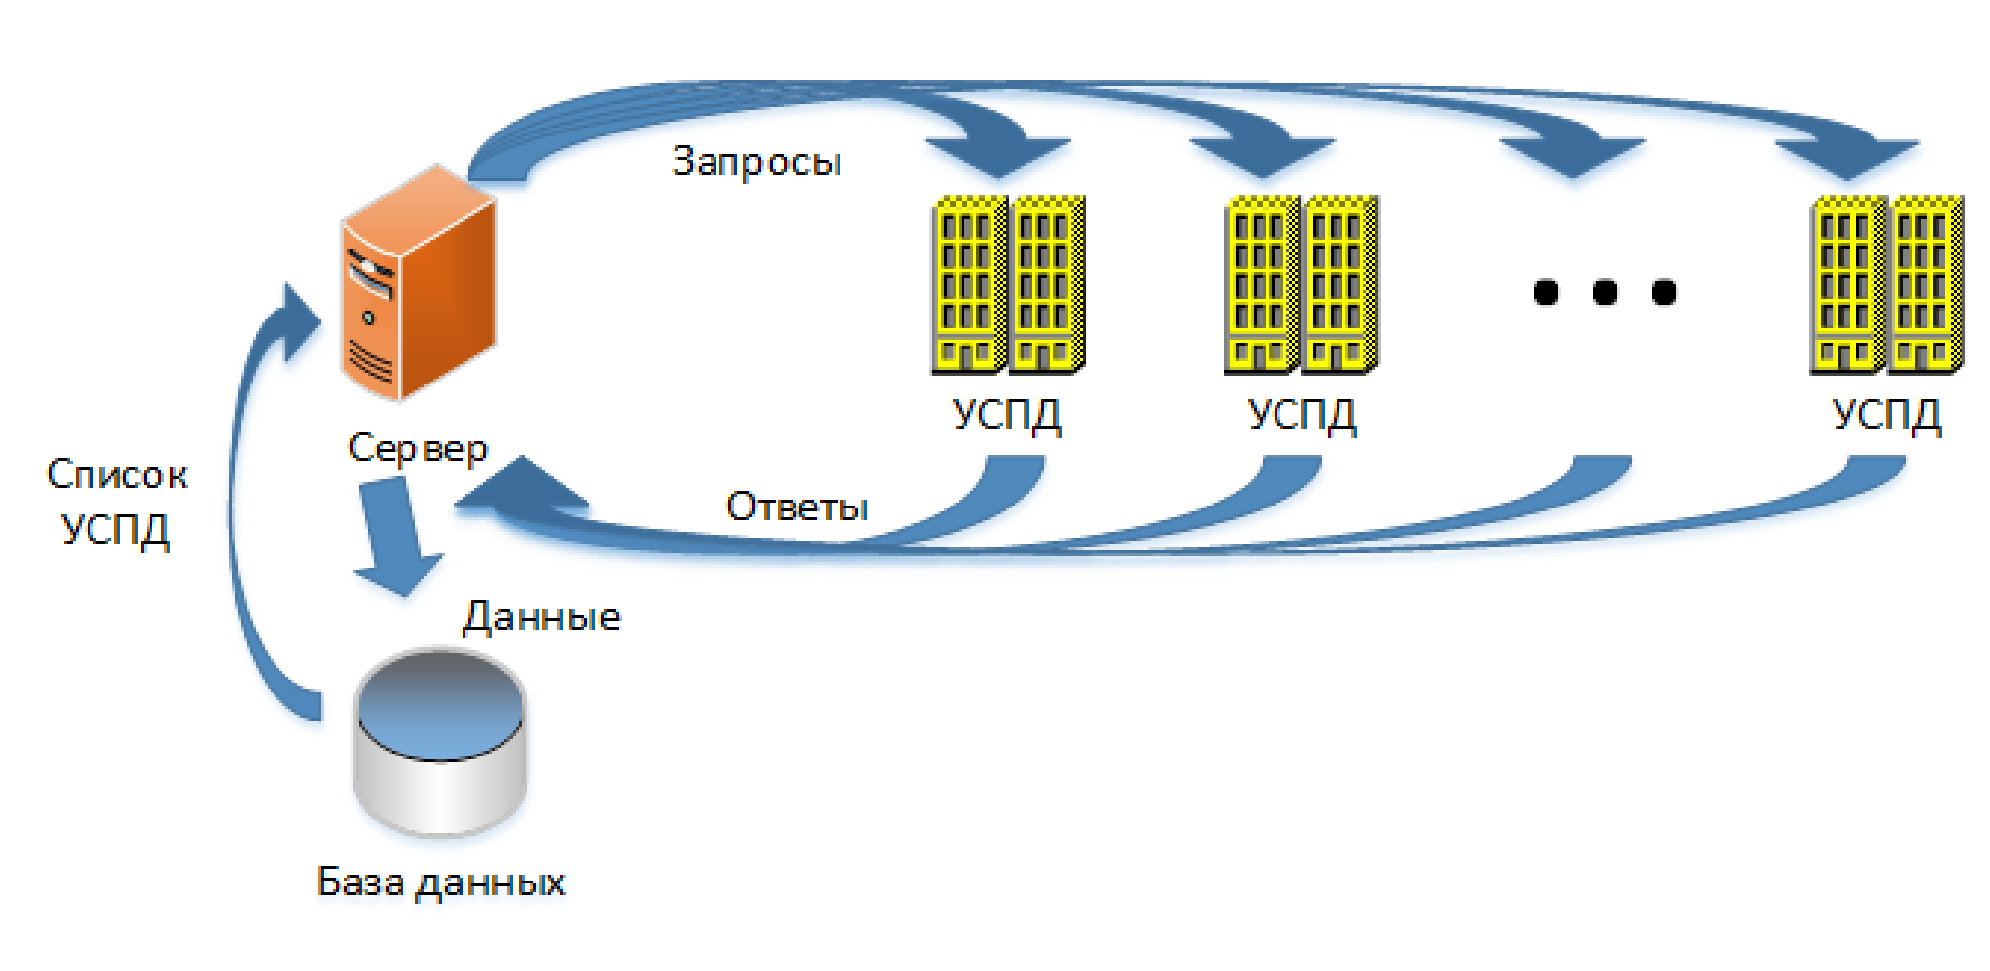
\includegraphics[width=0.8\linewidth]{scheme3}}
 \caption{Механизм взаимодействия с группой УСПД}
 \label{scheme3:scheme3}
\end{figure}

Процедура сбора данных с УСПД осуществляется на основании сформированных оператором правил опроса. Эти правила описывают в какое время и какое УСПД (или группу УСПД) необходимо опросить. В случае отсутствия правил опроса сбор данных производится по стандартной процедуре. Стандартная процедура сбора данных представляет собой последовательный опрос всего списка УСПД, зарегистрированных в системе. Сбор данных с УСПД может проводится в несколько потоков, то есть опрашивать одновременно несколько УСПД. Количество одновременно опрашиваемых УСПД указывается в настройках ССД.
В соответствии с вышеописанными правилами опроса формируются группы УСПД. Для каждой группы УСПД формируется две очереди опроса. Каждая очередь имеет свой временной интервал между опросами, указываемых в настройках ССД. Первая очередь содержит список опрашиваемой группы УСПД, вторая пуста. Из первой очереди происходит опрос УСПД. При успешном обращении к УСПД, оно удаляется из очереди, а в журнал заносится сообщение об успешном проведении операции. Если УСПД не отвечает, то оно переносится во вторую очередь. После опроса всех УСПД из первой очереди начинается опрос второй.
Данная очередь опрашивается несколько раз через небольшие промежутки времени. При ответе УСПД удаляется из очереди, а в журнал заносится сообщение о завершении операции с некоторыми проблемами. Если после последнего цикла опроса во второй очереди останутся УСПД, то о каждом из них в журнал заносится сообщение о неудачном завершении операции получения данных.
 \newpage
\section{Угрозы информации, передаваемой между УСПД и ССД}
\setcounter{figure}{0}

Информация, передаваемая от сервера сбора данных(ССД) к устройству сбора и передачи данных(УСПД) - это команды, которые обрабатывает УСПД. Информация, передаваемая от УСПД к ССД это показания устройств учета(УУ), статус УУ, статус УСПД. Передача информации происходит по глобальной сети интернет. Каналами может выступать проводное (ethernet) и беспроводное (GPRS) соединение.

\subsection{Виды угроз}

\begin{enumerate}
 \item угрозы нарушения физической целостности:
 \begin{itemize}
  \item разрушение каналов связи;
 \end{itemize}
 
 \item угрозы логической структуры:
 \begin{itemize}
  \item передача некорректных данных;
  \item ошибки адресации;
 \end{itemize}
 
 \item угрозы нарушения содержания:
 \begin{itemize}
  \item изменение передаваемой информации;
  \item получение поддельного пакета;
 \end{itemize}
 
 \item угрозы нарушения конфиденциальности:
 \begin{itemize}
  \item перехват идентификационных данных;
  \item перехват показаний пользователей;
 \end{itemize}
 
 \item угрозы нарушения прав собственности на информацию:
 \begin{itemize}
  \item подмена показаний;
  \item подмена идентификаторов УУ;
 \end{itemize}
 
\end{enumerate}

\subsection{Характеры возникновения угроз}

В таблице \ref{tab:threats_group} приведена классификация угроз по природе их возникновения.

\begin{center}
 \begin{longtable}[h!]{|*2{p{0.4\linewidth}|}}
  \caption{Классификация угроз} \label{tab:threats_group} \\
  \hline
  Естественные & Умышленные \\
  \hline
  разрушение каналов связи & передача некорректных данных\\
  \hline
  ошибки адресации & изменение передаваемой информации\\
  \hline
  передача некорректных данных & получение поддельного пакета\\
  \hline
  & перехват идентификационных данных\\
  \hline
  & перехват показаний пользователей\\
  \hline
  & подмена показаний\\
  \hline
  & подмена идентификаторов УУ\\
  \hline
  
 \end{longtable}

\end{center}


 \newpage
\section{Протоколы обмена данными в автоматизированных системах контроля}
\setcounter{figure}{0}

На рынке представлено множество датчиков, которые связываются с системой по различным протоколам. Используются такие протоколы как \cite{csp}:
\begin{itemize}
\item TCP/IP;
\item Modbus;
\item Canbus;
\item МЭК 60870-5-101;
\item МЭК 60870-5-104;
\item ОРС;
\item "Пирамида" (закрытый протокол);
\item спецпротоколы электросчетчиков;
\item SNMP;
\item TFTP;
\item RTU-325.
\end{itemize}

\subsection{Стандарт OPC}

OPC (OLE for Process Control) – семейство протоколов, предоставляющих единый интерфейс для управления объектами автоматизации и технологическими процессами. В частности, OPC DA (DataAccess) — стандарт, описывающий набор функций обмена данными в реальном времени с объектами автоматизации. 

Спецификация OPC охватывает:
\begin{itemize}
 \item концепцию клиент-серверную технологию OPC и определение данных;
 \item описания интерфейсов, методов, параметров и возможное их поведение;
 \item описание типов и структур данных;
 \item общие виды деятельности, которые включают в себя определение адресного пространства и его просмотра. Чтение, запись и подписка на уведомления об обновлении данных.
\end{itemize}

К недостаткам этого OPC можно отнести:
\begin{itemize}
 \item необходимость платного членства в сообществе The InteroperabilityStandard for Industrial Automation;
 \item протокол основан на технологиях windows.
\end{itemize}

Данный протокол не подходит, так как для его использования необходимо платное членство, что является неприемлемым для заказчика.

\subsection{Стандарт МЭК-60870-5-101/104}

МЭК-60870-5-101/104 – это протокол передачи данных, применяется в АСКТУ, АСКУЭ. Особенности реализации протокола МЭК 60870-101/104 при передаче данных между объектом и диспетчерским центром:

\begin{itemize}
 \item передача ограниченного количества информации, что обусловлено необходимостью переназначения всех сигналов с одного протокола на другой, и, как следствие, потеря некоторых данных, передача которых на этапе проектирования не была сочтена целесообразной;
 \item отсутствие единых наименований сигналов в рамках объекта и в центрах управления сетями, приводящее к сложности наладки и отслеживания ошибок;
 \item протокол МЭК 60870-5-101 предназначен для передачи данных по последовательным линиям связи RS-232/485;
 \item протокол МЭК 60870-5-104 является расширением протокола 101 и регламентирует использование сетевого доступа по протоколу TCP/IP.
\end{itemize}

Недостатки реализации данного стандарта:

\begin{itemize}
 \item количество передаваемых сигналов ограничивается определенным количеством дискретных входов и выходов;
 \item отсутствует возможность контроля связи между устройствами;
 \item возможно ложное срабатывание дискретного входа устройства при замыкании на землю в цепи передачи сигнала;
 \item цепи подвержены воздействию электромагнитных помех;
 \item сложность расширения систем;
 \item передача данных осуществляется в два этапа:
 \begin{enumerate}
  \item назначение индексированных коммуникационных объектов на прикладные объекты;
  \item  назначение прикладных объектов на переменные в прикладной базе данных или программе. Таким образом, отсутствует семантическая связь (полностью или частично) между передаваемыми данными и объектами данных прикладных функций.
 \end{enumerate}
 \item протоколы не предусматривают возможность передачи сигналов реального времени.
\end{itemize}

Данный протокол не подходит ввиду ограниченности возможностей и сложности масштабирования системы.

\subsection{Стандарт MODBUS}

Modbus – один из наиболее распространенных сетевых протоколов для интеграции устройств РЗА (релейная защита автоматики) в систему АСТУ, построенный на архитектуре «клиент–сервер». Данный протокол является открытым, что частично обуславливает его популярность. Протокол Modbus для передачи данных использует такие линиям связи как RS-485, RS-433, RS-232, а также сети TCP/IP (Modbus TCP).

Стандарт Modbus содержит в себе:

\begin{itemize}
 \item спецификация прикладного уровня;
 \item спецификация канального уровня;
 \item спецификация физического уровня;
 \item спецификацию ADU для транспорта через стек TCP/IP.
\end{itemize}

К достоинствам стандарта относится:

\begin{itemize}
 \item массовость;
 \item относительная простота реализации систем на его базе.
\end{itemize}

К недостаткам данного протокола можно отнести:

\begin{itemize}
 \item в случае необходимости отсутствует возможность оперативной сигнализации от конечного устройства к мастеру;
 \item стандарт не регламентирует начальную инициализацию системы. Назначение сетевых адресов и параметров системы для каждого устройства выполняются вручную на этапе адаптации;
 \item отсутствие  возможности  конечным  устройствам  обмениваться фиксированными данными друг с другом без участия мастера. Что ограничивает  применимость MODBUS-решений в системах регулирования реального времени.
\end{itemize}

Данный протокол не подходит ввиду отсутствия возможности оперативной сигнализации от конечного устройства к мастеру.

\subsection{Стандарт CAN}

CAN (Controller Area Network) – стандарт промышленной сети, использующийся для объединения в единую сеть устройств и датчиков. Применяется в системах автоматизации промышленного производства. 

В первую очередь данный стандарт описывает физический уровень, наибольшую популярность получил вариант описанный в ISO 11898-2. Физический уровень использует дифференциальную передачу данных по витой паре, для управления доступом к шине используется неразрушающее bit-wise разрешение конфликтов ISO 11898.

К положительным аспектам данной реализации относиться:

\begin{itemize}
 \item работа в режиме жёсткого реального времени;
 \item высокая устойчивость к помехам;
 \item надёжный контроль ошибок приема-передачи данных.
\end{itemize}

К достоинствам данного стандарта относятся:

\begin{itemize}
 \item сообщения имеют малые размеры (8 байт данных) и защищены контрольной суммой;
 \item большой размер служебных данных в пакете по отношению к полезным данным;
 \item отсутствие единого общепринятого стандарта на протокол высокого уровня (в том числе TCP).
\end{itemize}

Данный протокол не подходит из-за сложностей использования в сетях интернет.

\subsection{Стандарт DLMS}

DLMS (Device Language Message Specification) – стек протоколов, ориентированный на 16-разрядные микроконтроллеры Microchip PIC. Является международным стандартом для систем сбора данных с электро-, газовых, водяных и тепловых счетчиков. Работает на основе протоколов связи (RS232, RS485, PSTN, GSM, GPRS, IPv4, PPP и PLC), с поддержкой шифрования AES128.

Особенности данного протокола:

\begin{itemize}
 \item работает на всех 16-битных микроконтроллерах PIC и dsPIC;
 \item возможность интеграции стека DLMS с текущими реализациями протоколов TCP/IP, ZigBee и PLC;
 \item небольшой объем занимаемой памяти позволяет использовать компактные и недорогие контроллеры;
 \item для европейского рынка стек поддерживает IEC 62056-21 Mode E.
\end{itemize}

К недостаткам данного протокола можно отнести то, что описание протокола предоставляется на платной основе или требуется членство в ассоциации DLMS. Что является неприемлемым для заказчика.

Из представленного краткого анализа видно, что существующие протоколы связи достаточно успешно позволяют реализовывать задачи диспетчерского управления / интеграции данных в системы управления, однако не все они позволяют реализовывать функции реального времени. К тому же большое количество проприетарных протоколов приводит к усложнению процесса интеграции устройств в единую систему: 

\begin{itemize}
 \item протоколы должны поддерживаться контроллером, что требует реализации поддержки большого количества протоколов в в нем и ведет к удорожанию оборудования;
 \item для интеграции устройств по проприетарным протоколам требуется квалификация наладочного персонала в работе с каждым из них;
 \item переназначение сигналов из проприетарных протоколов в общепромышленные и назад часто приводит к потере информации, включая дополнительную информацию;
 \item при передаче данных по-прежнему применяется большое количество последовательных интерфейсов, что накладывает ограничения на скорость передачи данных, объем передаваемых данных и количество устройств, одновременно включенных в информационную сеть.
\end{itemize}

\subsection{Предлагаемое решение}

Большинство приборов учета (или УСПД) поддерживают протокол передачи данных TCP/IP, в виду чего использование данного протокола на транспортном уровне является целесообразным, так как в отличие от других протоколов передачи данных TCP/IP имеет следующие преимущества:

\begin{itemize}
 \item скорость разработки и цена разработки;
 \item использование в сетях интернет;
 \item более простой (простая поддержка);
 \item обеспечивает контроль целостности передаваемых данных;
 \item возможность обеспечить программную поддержку новых устройств через модульную систему драйверов.
\end{itemize}

TCP (англ. Transmission Control Protocol, протокол управления передачей) — один из основных протоколов передачи данных Интернета, предназначенный для управления передачей данных в сетях и подсетях TCP/IP\cite{tcp}.

Для обеспечения защищенного соединения необходимо использовать технологии построения виртуальных каналов. 

Технология построения защищенного соединения в открытых сетях так же позволит решить проблему конфиденциальности передаваемых данных благодаря тому, что весь передаваемый трафик передается в шифрованном виде. Примером таких технологий является технология VPN. VPN (англ. Virtual Private Network — виртуальная частная сеть\cite{vpn}) — обобщённое название технологий, позволяющих обеспечить одно или несколько сетевых соединений (логическую сеть) поверх другой сети (например, Интернет). Несмотря на то, что коммуникации осуществляются по сетям с меньшим или неизвестным уровнем доверия (например, по публичным сетям), уровень доверия к построенной логической сети не зависит от уровня доверия к базовым сетям благодаря использованию средств криптографии (шифрования, аутентификации, инфраструктуры открытых ключей, средств для защиты от повторов и изменений передаваемых по логической сети сообщений).

Так же для решения данной задачи возможно использование технологии SSH. SSH (англ. Secure Shell — «безопасная оболочка»\cite{ssh}) — сетевой протокол прикладного уровня, позволяющий производить удалённое управление операционной системой и туннелирование TCP-соединений (например, для передачи файлов). Схож по функциональности с протоколами Telnet и rlogin, но, в отличие от них, шифрует весь трафик, включая и передаваемые пароли. SSH допускает выбор различных алгоритмов шифрования. SSH-клиенты и SSH-серверы доступны для большинства сетевых операционных систем. 

Тогда последовательность действий при запросе данных от ССД к УСПД имеет следующий вид:

\begin{enumerate}
 \item установление соединения между ССД и УСПД;
 \item отправка идентификационных данных ССД на УСПД;
 \item отправка запроса на получение данных от УСПД;
 \item получение данных от УСПД;
 \item завершение соединения.
\end{enumerate}

Функциональная схема данного процесса представлена на рисунке \ref{img:get_data_idef0}.

\begin{figure}[!ht]
 \center{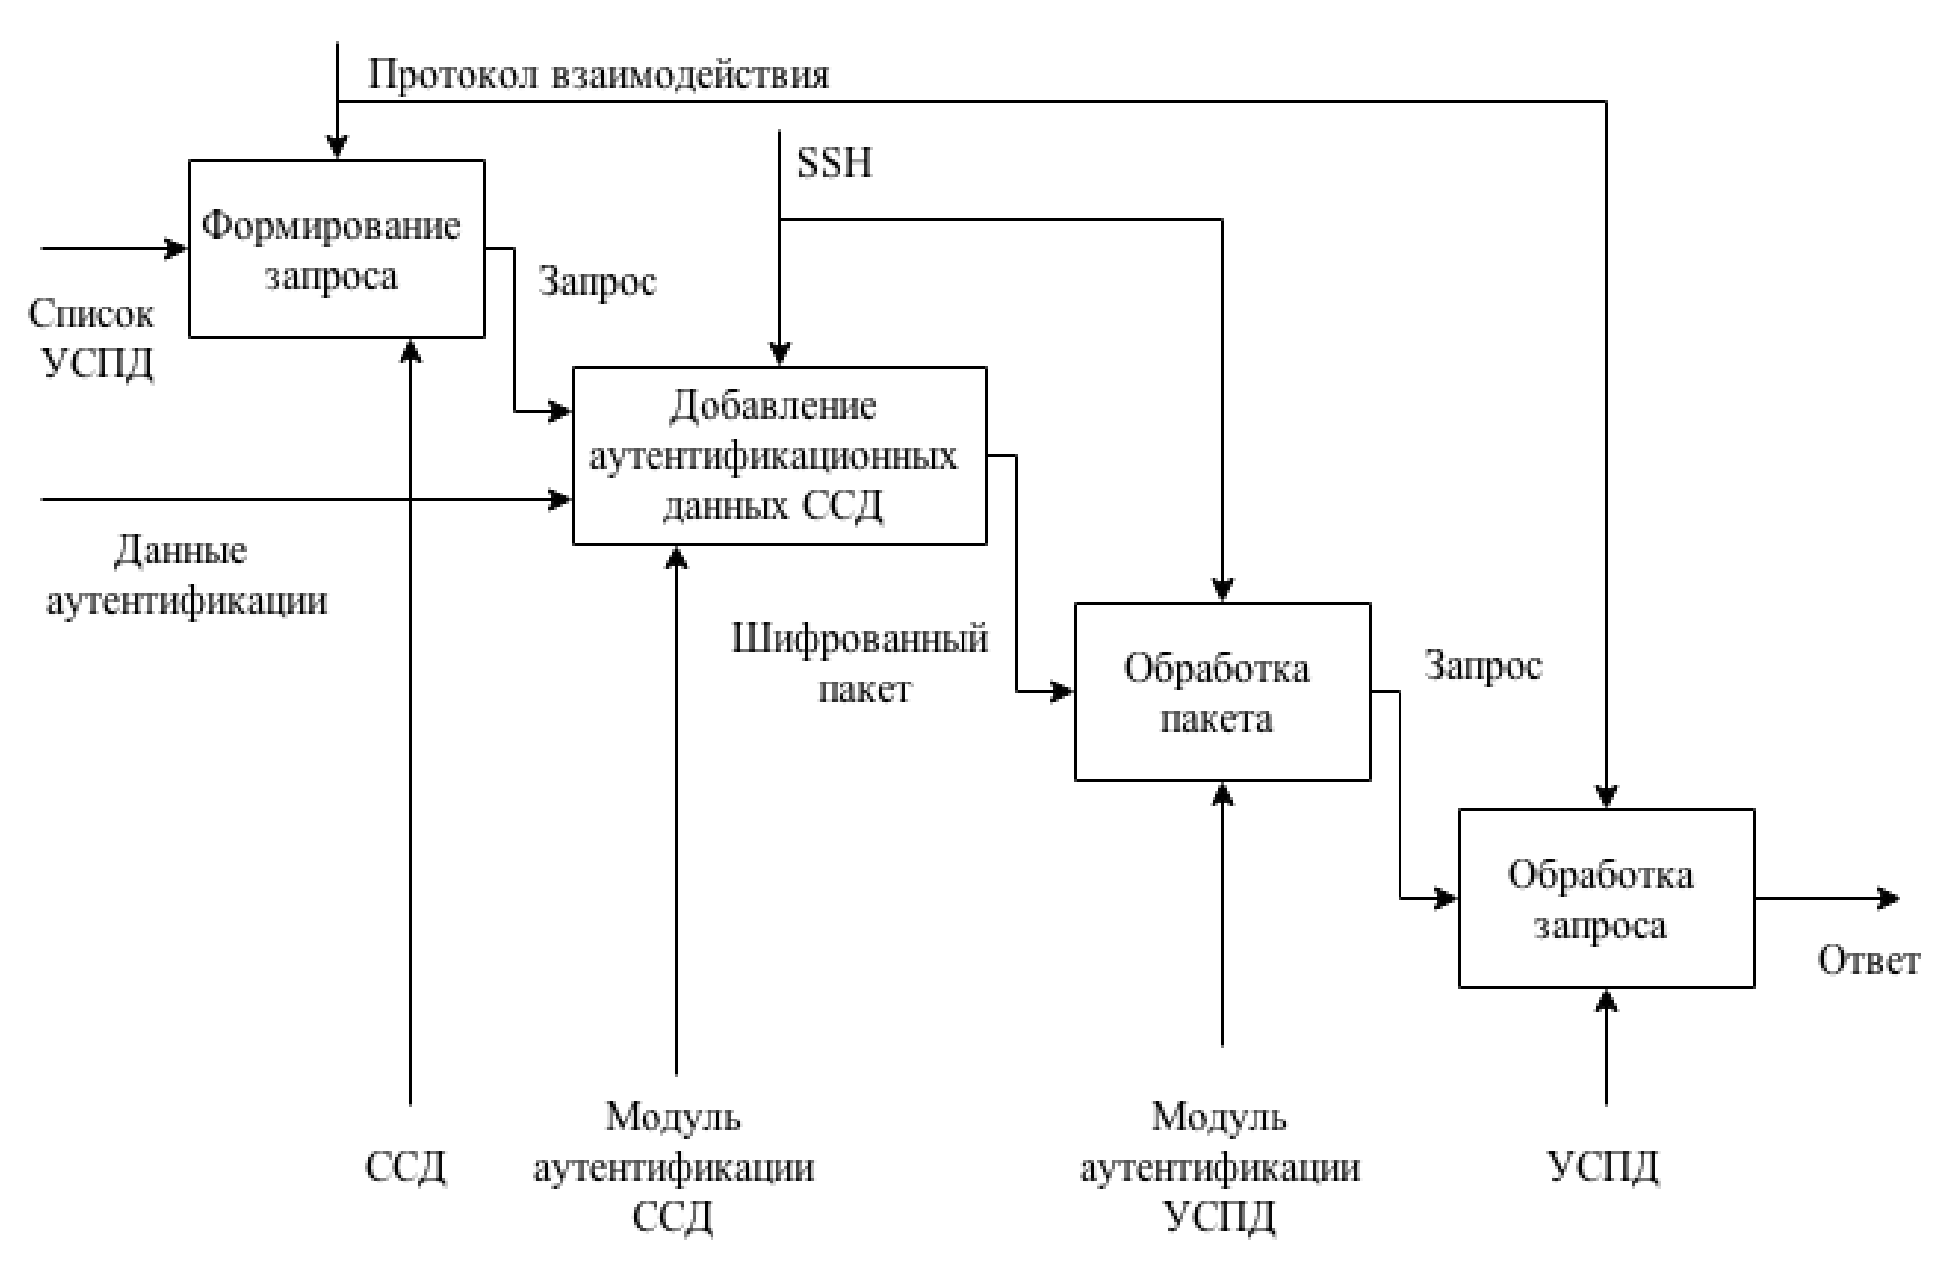
\includegraphics[width=0.8\linewidth]{get_data_idef0}}
 \caption{Запрос данных с УСПД}
 \label{img:get_data_idef0}
\end{figure}

Использование технологий построения виртуальных частных каналов позволяет защититься от угроз:

\begin{itemize}
 \item внедрение ложного объекта сети;
 \item анализ сетевого трафика;
 \item подмена доверенного объекта;
 \item навязывание ложного маршрута;
 \item выведывание паролей.
\end{itemize}

 \newpage
\section{Механизмы защиты}
\setcounter{figure}{0}

При разработке мехнаизма взаимодействия необходимо учесть следующие проблемы:
\begin{itemize}
 \item надежнось передачи данных;
 \item контроль устройств, передающих информацию на ССД;
 \item конфиденциальность передаваемой информации.
\end{itemize}

\subsection{Обеспечение надежной передачи данных} %Для осуществления передачи данных между ССД и УСПД самым простым вариантом является передача данных через сеть интернет. Передача данных по протоколу TCP обеспечит надежность передачи данных, а так же освободит от задачи разработки транспортных механизмов данных в линиях связи.


Под надежностью передачи понимается гарантированная доставка данных от УСПД на ССД. То есть, что все сообщения будут получены без каких либо искажений и потерь. В стеке протоколов TCP/IP на транспортном уровне используется протокол TCP. TCP (англ. Transmission Control Protocol, протокол управления передачей) — один из основных протоколов передачи данных Интернета, предназначенный для управления передачей данных в сетях и подсетях TCP/IP.[4]

Механизм TCP предоставляет поток данных с предварительной установкой соединения, осуществляет повторный запрос данных в случае потери данных и устраняет дублирование при получении двух копий одного пакета, гарантируя целостность передаваемых данных благодаря помехоустойчевому кодированию с возможностью восстановления и уведомление отправителя о результатах передачи.

Использование протокола ТСР на транспортном уровне освобождает от задачи реализации своих механизмов передачи данных и позволяет использовать сети интернет для обмена данными. Это позволит сократить время разработки и способствует решению проблемы с линиями связи между УСПД и ССД. 

При таком подходе будут использоваться линии связи, подведенные в здания интернет-провайдерами, либо выход в сети интернет будет придоставлен при помощи GPRS-модемов. 

\subsection{Контроль подключаемых устройств} %При изучении существующих протоколов было отмечено что в существующих системах УСПД и серверы являлись равнозначными, в разрабатываемой системе предлагается отказаться от данной концепции и сделать УСПД ведомым устройством, то есть отдавать данные только по запросу от ССД. Благодаря такому подходу не будет возможности отправить поддельный пакет на ССД. На УСПД же необходимо хранить идентификационные данные сервера для контроля подключений к УСПД. 

\subsection{Обеспечение конфиденциальности передаваемых данных} %Для обеспечения конфиденциальности передаваемой информации по откртым сетям необходимо использовать технологии построения виртуальных шифрованных каналов связи, таких как VPN.


 %TODO механизмы защиты от угроз
 \newpage
\section{Механизм взаимодействия сервера сбора данных с УСПД}
\setcounter{figure}{0}

В разрабатываемой системе сервер является инициатором всех обменов данными, а клиенты ожидают запроса для передачи данных. Схема взаимодействия приведена на рисунке \ref{scheme2:scheme2}.

\begin{figure}[h!]
 \center{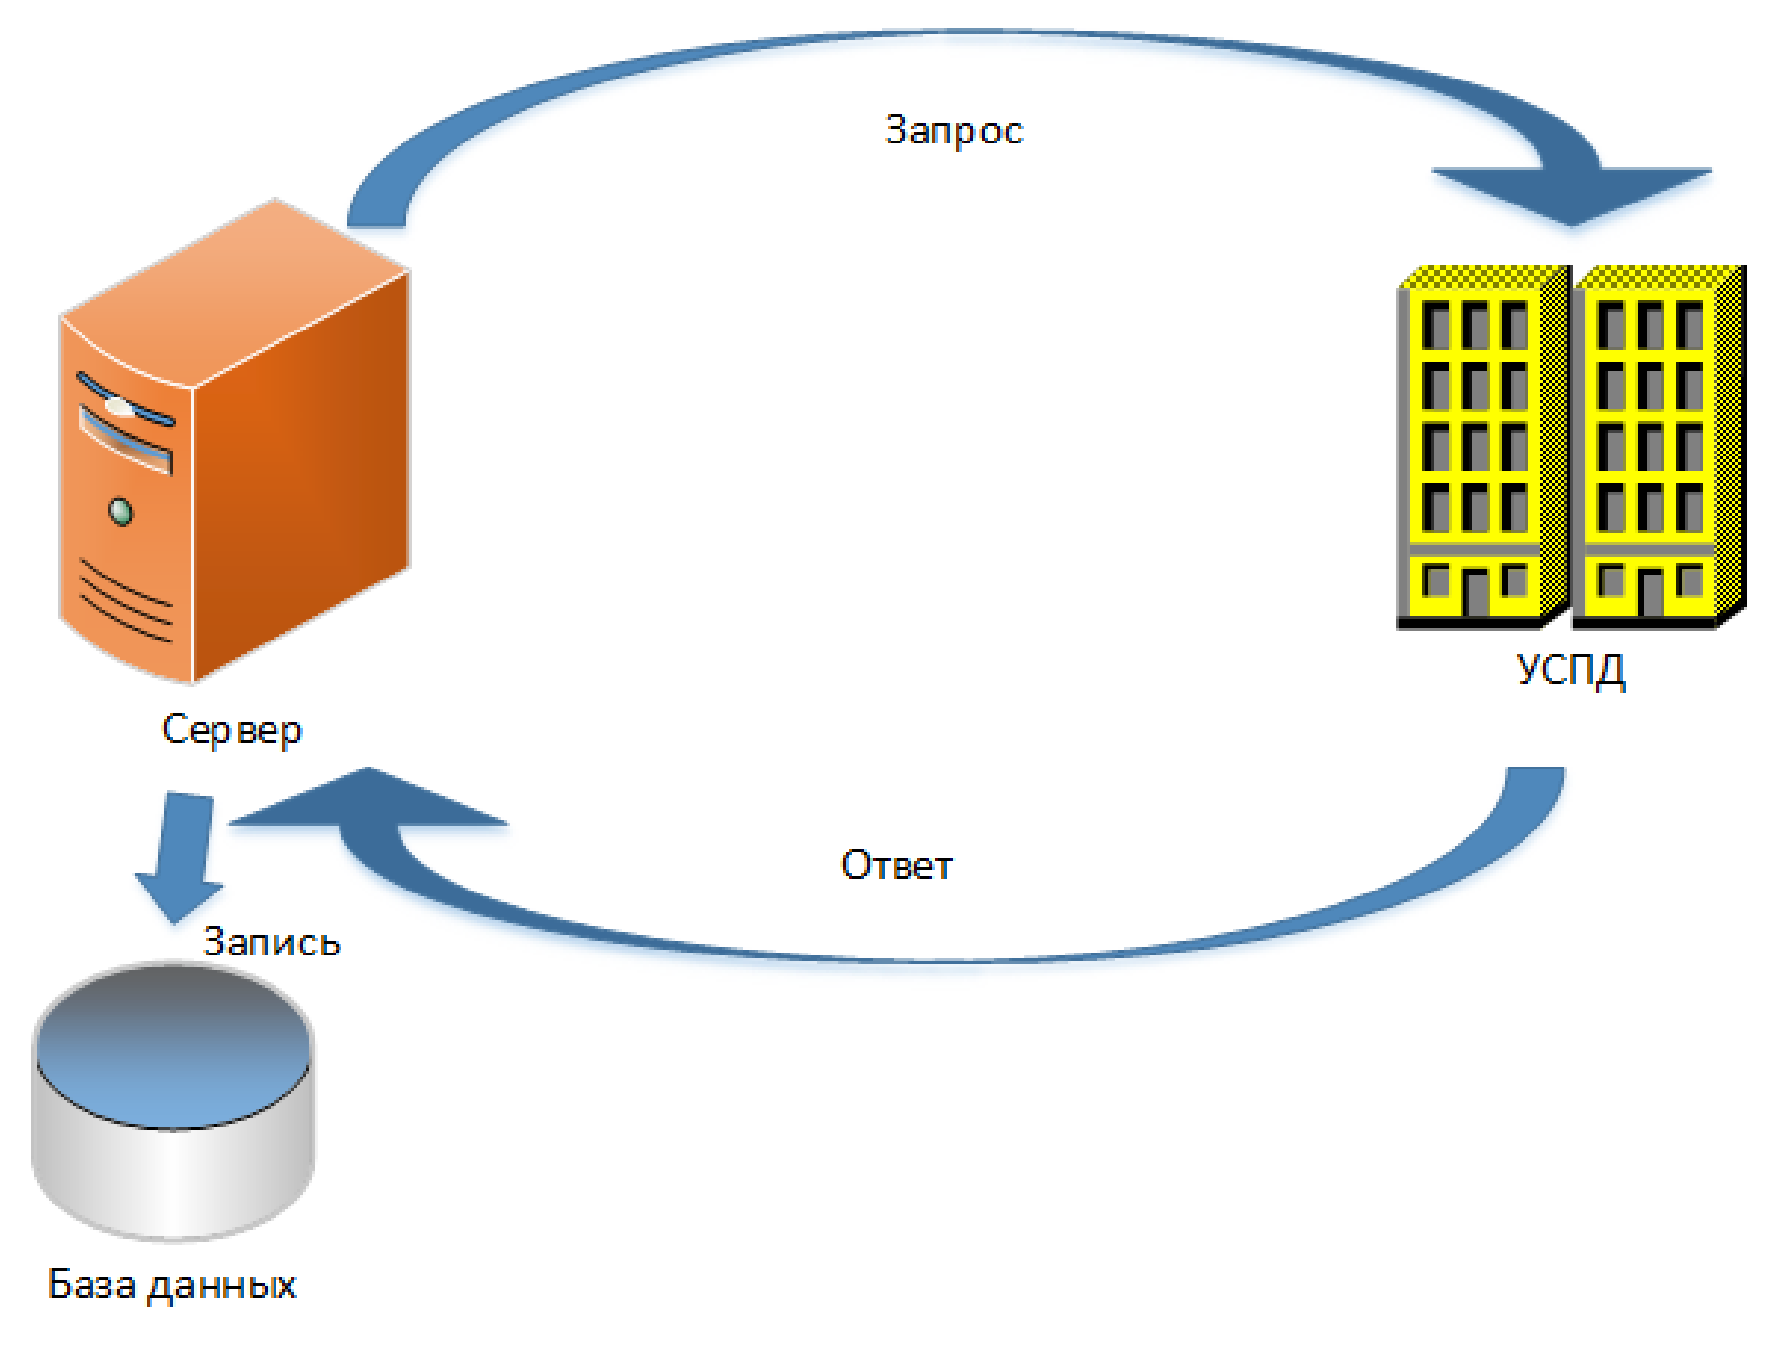
\includegraphics[width=0.8\linewidth]{scheme2}}
 \caption{Схема взаимодействия сервера с УСПД}
 \label{scheme2:scheme2}
\end{figure}

Данный механиз позволяет реализовать опрос УСПД по списку, хранящемуся на сервере, что исключит возможность отправки данных с несанкционированных устройств. Так же появляется возможность обнаружения неисправности УСПД либо ошибки сети, на который сервер будет реагировать предупреждениями. 

Данные, полученные с УСПД, записываются во временную базу данных для последующей обработки и отправки на центральный сервер. В этой же базе данных хранится список всех УСПД, подконтрольных данному серверу. Схема представлена на рисунке \ref{scheme3:scheme3}.

\begin{figure}[h!]
 \center{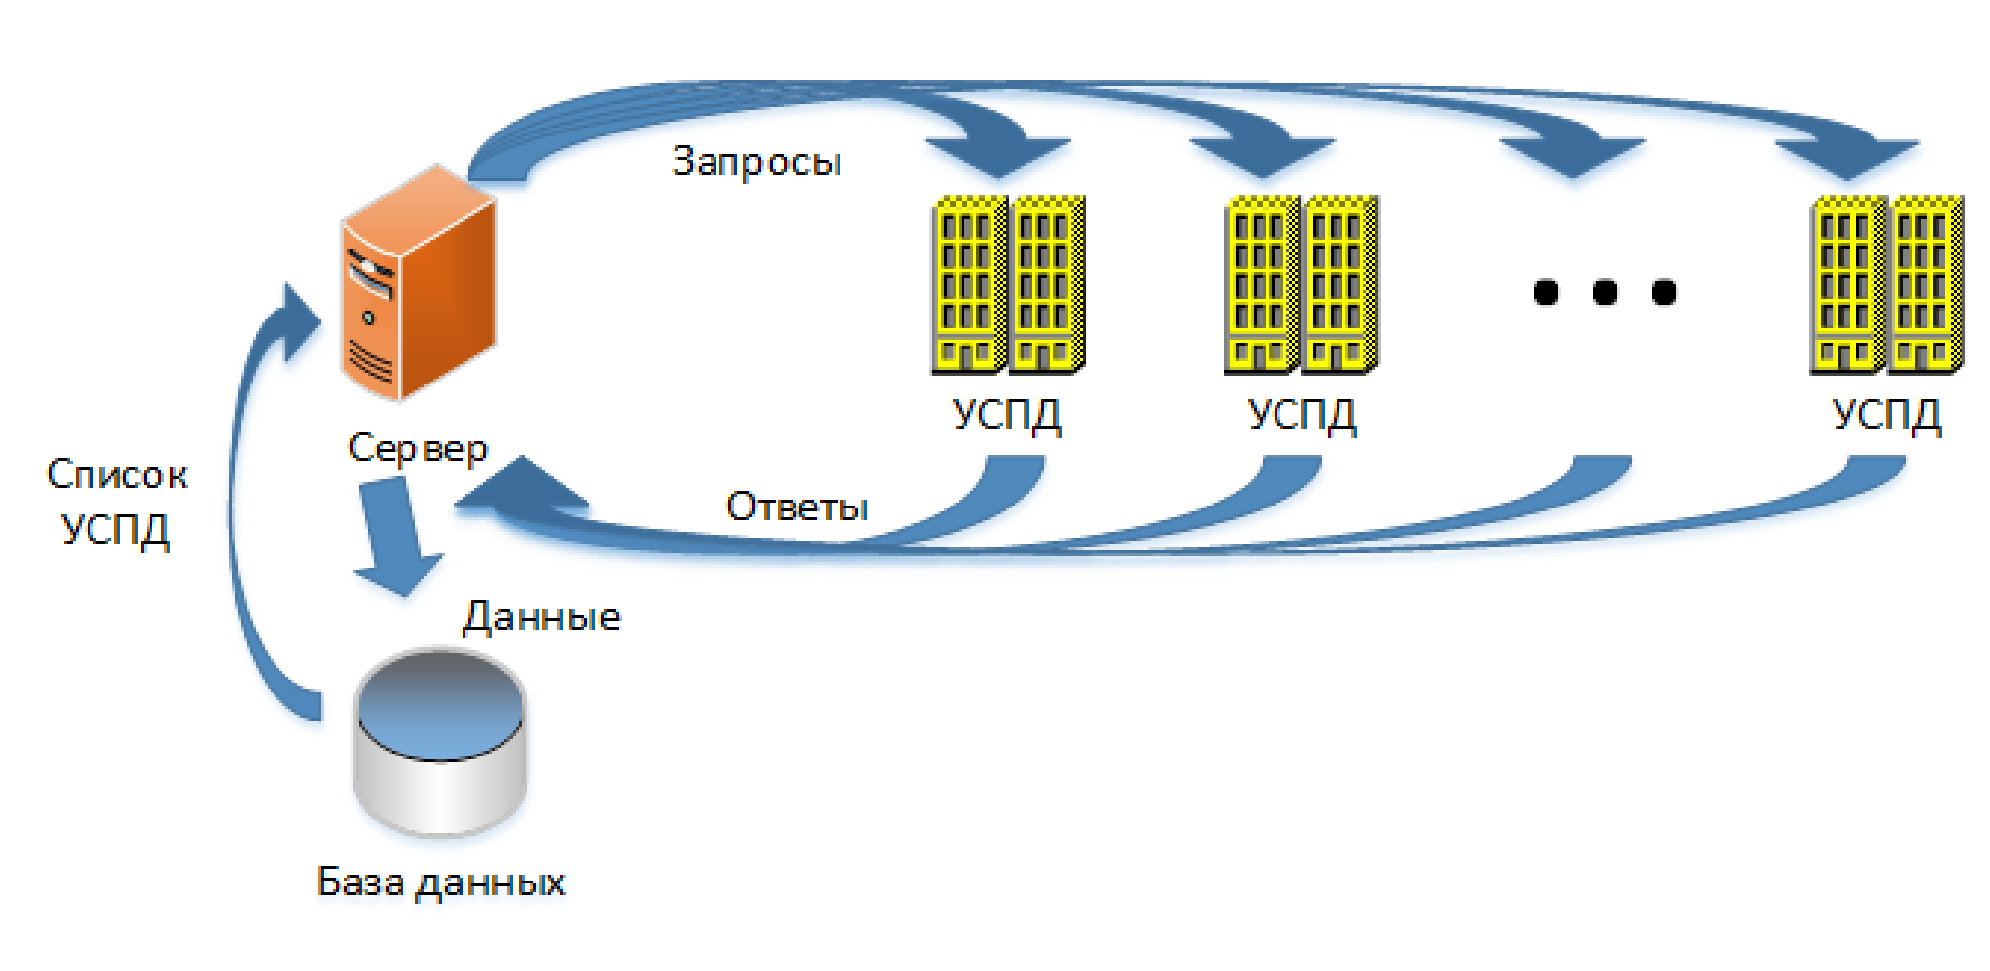
\includegraphics[width=0.8\linewidth]{scheme3}}
 \caption{Механизм взаимодействия с группой УСПД}
 \label{scheme3:scheme3}
\end{figure}

 \section{Сетевое взаимодействие}

Было принято решение реализовывать взаимодействие УСПД и центрального сервера по протоколу TCP/IP.

Механизм TCP предоставляет поток данных с предварительной установкой соединения, осуществляет повторный запрос данных в случае потери данных и устраняет дублирование при получении двух копий одного пакета, гарантируя тем самым целостность передаваемых данных и уведомление отправителя о результатах передачи.

\subsection{Сетевое взамодействие в Qt Framework}

Сетевое взаимодействие в программах, реализованных на языке C++ реализуется при помощи сокетов, в Qt для реализации данного взаимодействия используется надстройка над механизмом сокетов, облегчающая реализацию данного взаимодействия.

Данный механизм представлен такими классами как \cite{qt_net}:
\begin{itemize}
 \item QAbstrackSocket;
 \item QTcpSocket;
 \item QTcpServer;
 \item QUdpSocket.
\end{itemize}

Для реализации взаимодействия будут использоваться классы QTcpSocket и QTcpServer.

\subsection{УСПД}

Для тестирования разрабатываемой программы был сделан эмулятор, на базе одноплатного компьютера Raspberry Pi B+. 

Для данного компьютера был написан скрипт на языке python. Задачей скрипта является открыть порт на устройстве и реагировать на все данные, приходящие на этот порт отправкой данных в обратном порядке. 

Текст скрипта:

\begin{lstlisting}
#!/usr/bin/python
# -*- coding: utf-8 -*-

import socket

sock = socket.socket()
sock.bind(('', 9090))
sock.listen(5)
while True:
        conn, addr = sock.accept()
        while True:
                data = conn.recv(1024)
                if not data:
                        break
                buf = data[::-1] + '\n'
                print data
                conn.send(buf)

conn.close()
\end{lstlisting}

\subsection{Взаимодействие с УСПД}

В первую очередь необходимо реализовать функцию оптравки данных по сети. 

Для этого был создана программа с графическим итерфейсом. Задачей данной программы является установление соединения с определенным адресом и получением/отправкой текстовой информации.

Прототип объекта, решающего эту задачу, выглядит так:

\begin{lstlisting}
class EmulSocket : public QObject
{
    Q_OBJECT
public:
    explicit EmulSocket(QObject *parent = 0);
    ~EmulSocket();
    void configure(QString, int);
    void initSocket();
    void sendData(QByteArray);

private:
    QString qs_Address;
    int i_Port;
    QTcpSocket * sc;
signals:
    void haveData(QString);
public slots:
    QString getData();
};
\end{lstlisting}

В конструкторе и диструкторе объекта инициализируется и уничтожается объект QTcpSocket *sc.

Метод configure(QString, int) заполняет значения ip-адреса и порта назначения (поля qs\_Address и i\_Port соответственно), так же в данном методе происходит связывание события ``приняты данные'' с обработчиком этого события - методом getData(). После чего вызывается метод initSocket().

Метод initSocket() отвечает за установление соединения с указанным хостом.

Метод sendData(QByteArray) - это функция, отправляющая полученный массив байт по адресу назначения.

Сигнал haveData(QString) - это вспомогательный сигнал для взаимодействия объекта с графическим интерфейсом.

Метод getData() обрабатывает входящий поток данный и при получении данных испускает сигнал haveData(QString) в котором передает полученные данные.

Интерфейс программы представлен на рисунке \ref{window1:window1}.

\begin{figure}[h!]
 \center{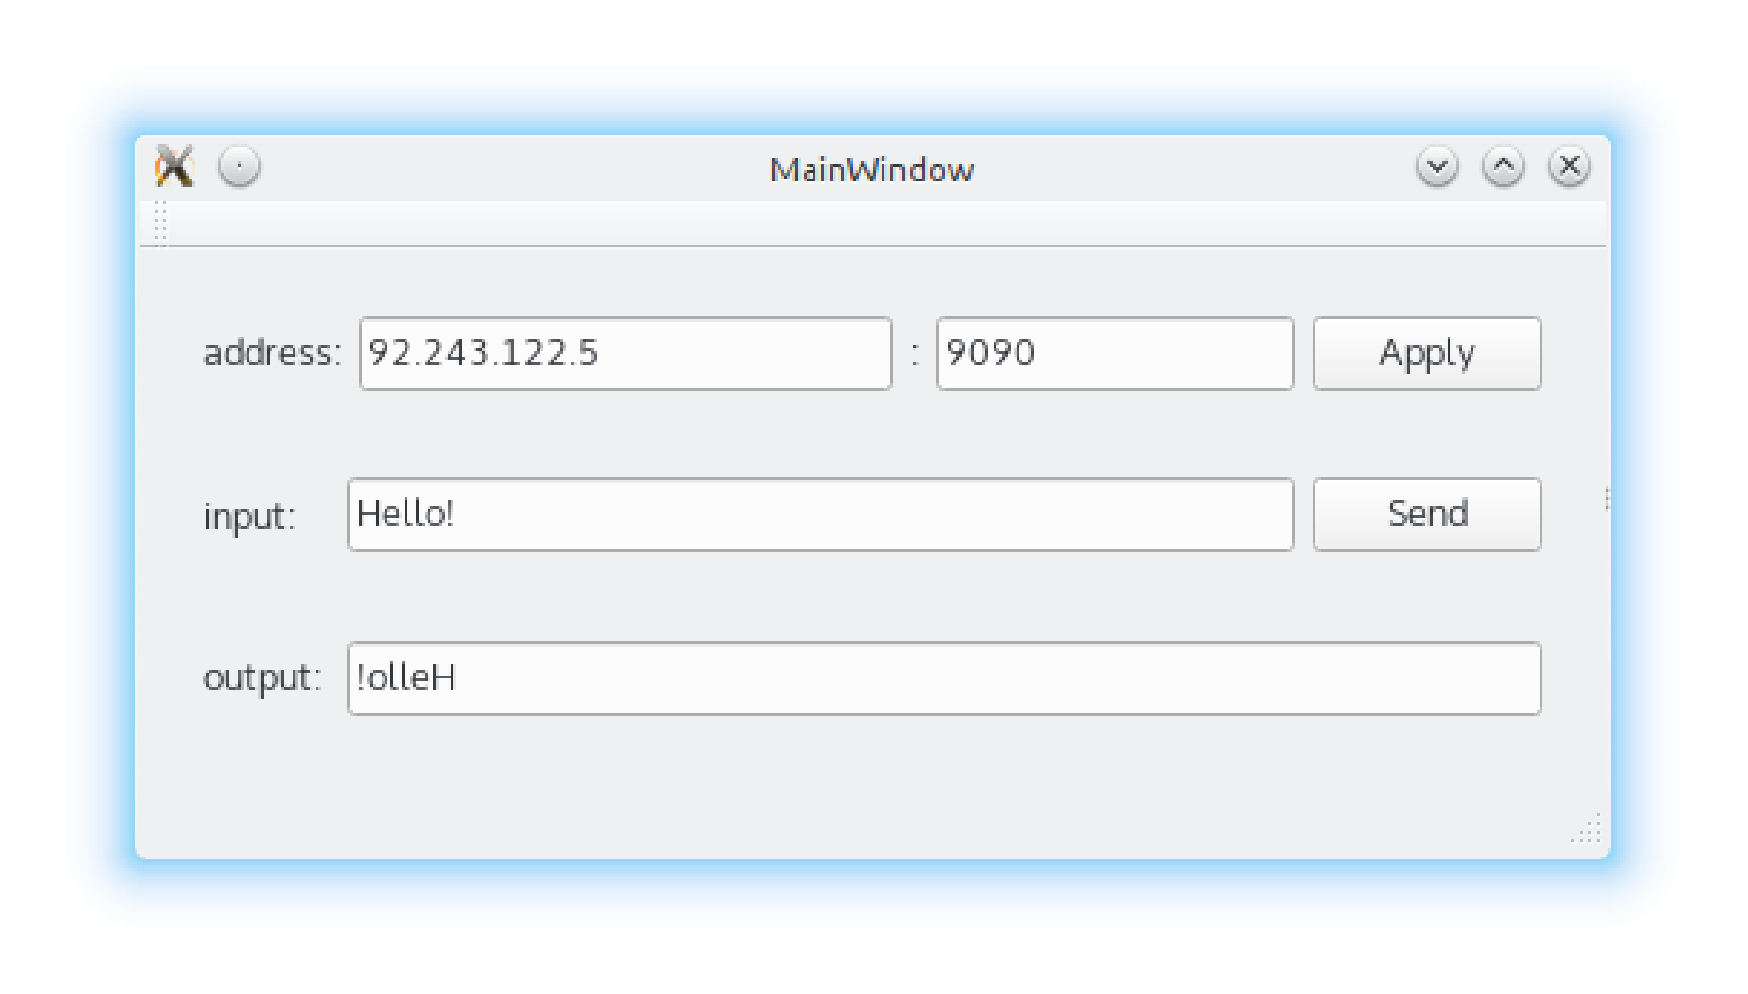
\includegraphics[width=0.7\linewidth]{window1}}
 \caption{Подключение к эмулятору УСПД}
 \label{window1:window1}
\end{figure}

\subsection{Сохранение данных}

После установления связи с УСПД необходимо фиксировать полученную информацию в базе данных. Для теста была выбрана СУБД SQLite. 

Необходимо записывать в базу данных все ответы с эмулятора, при этом дописывать к ним время получения.

В базе данных создана одна таблица с тремя полями: id, data, time.

Для реализации данного функционала необходимо реализовать функции для работы с базой данных. Для этого в реализованном ранее приложении был добавлен новый объект. 

Описание объекта:

\begin{lstlisting}
class EmulDB : public QObject
{
    Q_OBJECT
public:
    explicit EmulDB(QObject *parent = 0);
    ~EmulDB();

    bool dbConnect(const QString& );
    void dbDisconnect();
    bool dbInsert(const QString& );

private:
    QSqlDatabase m_db;
    bool m_bOpen;
};
\end{lstlisting}
Конструктор и диструктор не выполняют каких либо дополнительных действий, атрибуты m\_db и m\_bOpen это база данных и её состояние (подключена ли база данных) соответственно.

Методы dbConnect и dbDisconnect необходимы для подключения и отключения к базе даных. 

Метод dbInsert принимает данные и записывает их в таблицу, подставляя время записи.

На рисунке \ref{dBase:dBase} представлено содержимое базы данных после тестового запуска программы.

\begin{figure}[h!]
 \center{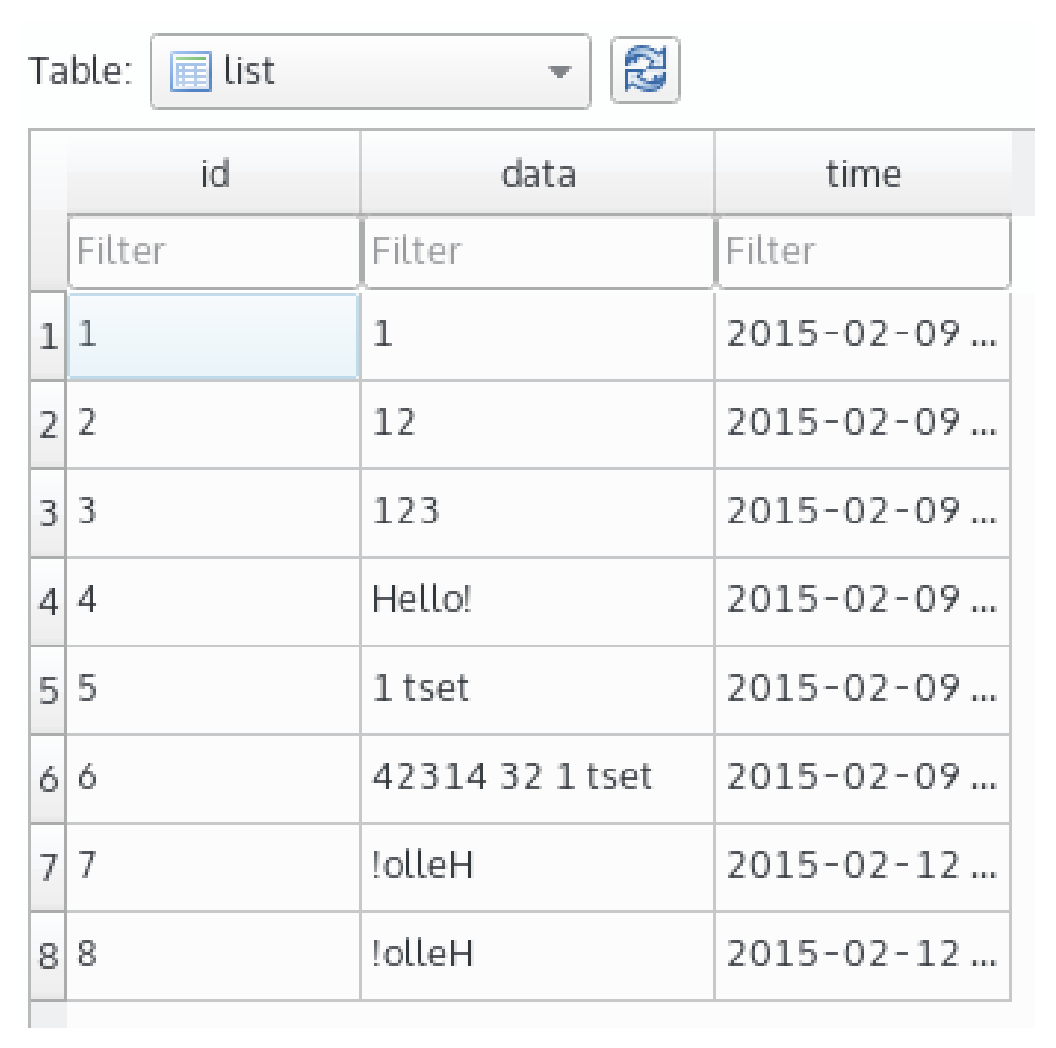
\includegraphics[width=0.7\linewidth]{dBase}}
 \caption{Просмотр таблицы}
 \label{dBase:dBase}
\end{figure}
 \section{Сервер сбора данных}
\subsection{Постановка задачи}

В первую очередь необходимо реализовать функции опроса клиентов. Так же программа должна обладать информацией о клиентах, тоесть иметь список данных клиентов, в которых содержится адрес клиента (ip-адрес и номер порта).

Так же для тестировани необходим более сложный эмулятор, который бы поддерживал несколько параллельный подключений с выводом информации о появлении нового подключения, разрыве соединения и отображения полученной информации.

\subsection{Приложение-клиент}

Так как это вспомогательное приложение, для простоты разработки не будем создавать для него графический интерфейс. 

Идея состоит в том, что бы создать приложение которо ожидает подключения и при появлении такового создает новое tcp соединение и принимает информацию, так же приложение должно проверять статус соединения и при его разрыве удалять созданные сокеты для освобождения портов. Данный механизм в дальнейшем будет использоваться и на сервере.

Для ожидания соединения нам нужно создать специальный объект, которы реагировал бы на обращение к определенному порту клиентской машины. Для создания такого объекта воспользуемся классом QTcpServer. Данный класс порождает объекты, которые, прослушивающие порт и испускающие сигналы при появлении запроса на соединение.

Создадим класс TestServ. Прототип класса представлен ниже.

\begin{lstlisting}
class TestServ : public QObject
{
    Q_OBJECT
public:
    explicit TestServ(QObject *parent = 0);
    ~TestServ();

    void initServ(const int &port);

private:
    QTcpServer *srv;
    QMap<QString, ClientSock*> users;
signals:

public slots:
    void newConnection();
    void connectClosed(QString name);
};
\end{lstlisting}
В конструкторе и диструктора класса инициилизируется объект srv, так же в конструкторе связывается сигнал объекта srv newConnection со слотом данного класса newConnection.

Метод initServ указывает объекту srv какой порт необходимо прослушивать, и выводит в консоль информацию о том, успешно ли прошел запуск сервера.

QMap<QString, ClientSock*> users - это контейнер для хранения указателей на созданные в даный момент сокеты с присвоенными им именами.

Слот newConnection() отрабатывает при появлении нового запроса на соединение, здесь в консоль выводится сообщение о создании нового запроса и создается и инициализируется объект ClientSock*, после чего его сигнал scDisconnect(QString) связывается со слотом connectClosed(QString) и указатель помещается в QMap.

Слот connectClosed принимает на вход имя слота, производит поиск укзателя с данным именем, отдает команду уничтожить объект и удаляет запись о данном объекте из QMap.

Объект ClientSock это ранее созданный класс EmulSock с добавлением нескольких методов и сигналов. Прототип данного класса представлен ниже.

\begin{lstlisting}
class ClientSock : public QObject
{
    Q_OBJECT
public:
    explicit ClientSock(QObject *parent = 0);
    explicit ClientSock(QTcpSocket *sock, QObject *parent = 0);
    ~ClientSock();
    void initSc(const QString & addr, const int & port);
    void setName(const QString & name);
    QString getName();
    void sendData(QByteArray data);
    void timerEvent(QTimerEvent *event);
private:
    QTcpSocket * sc;
    QString m_qsScName;
signals:
    void scDisconnect(QString);
public slots:
    QByteArray getData();
};
\end{lstlisting}

В описании добавился конструктор, принимающий указатель на объект QTcpSocket, необходимый для создания объекта на основании данных, полученных от объекта srv.

Методы getName и setName необходиы для работы с атрибутом m\_qsScName, хранящую имя объекта.

Метод timerEvent необходим для отслеживания статуса сокета sc, данный метод вызывается всякий раз при обнулении таймера, запускаемого при создании объекта типа ClientSock в констукторе. Данный метод проверяет статус сокета и при получении статуса ``отключен'' останавливате таймер, выводит сообщение о прекращении соединения и испускает сигнал что соединение закрыто, который обрабатывается объектом типа TestServ.

В функции main просто создаем объект типа TestServ, и указываем ему порт назначения, переданный первым аргументом при запуске программы. Пример работы с подключением одного клиента представлен на рисунку \ref{clientEmul:clientEmul}.

\begin{figure}[h!]
 \center{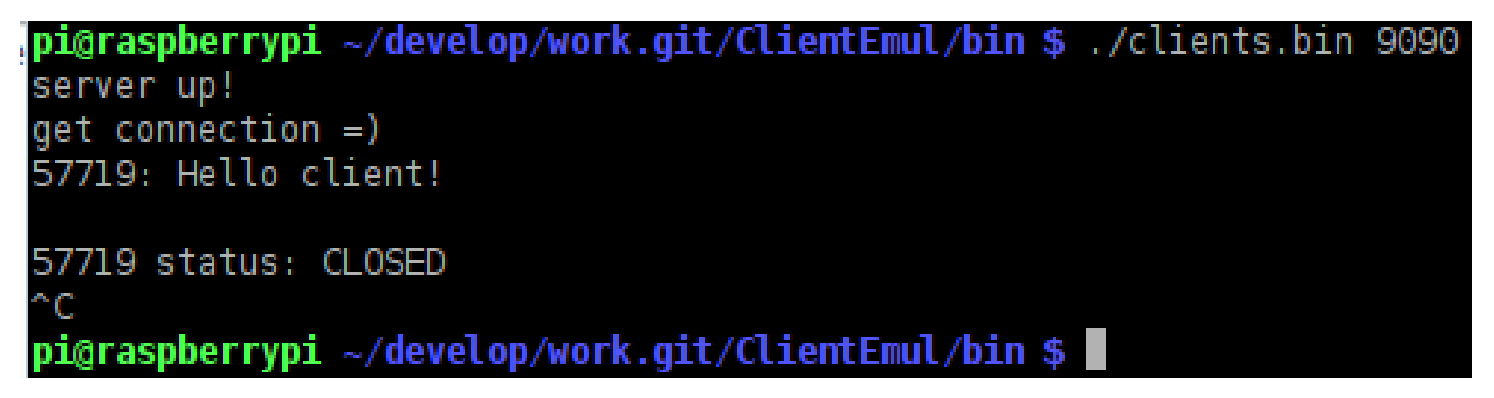
\includegraphics[width=0.7\linewidth]{clientEmul}}
 \caption{Демонстрация работы приложения}
 \label{clientEmul:clientEmul}
\end{figure}

 \newpage
 %TODO
 \input{teo} %TODO экономика
 \newpage
\section{Разработка вопросов охраны труда}
\setcounter{table}{0}

В соответствии с ГОСТ 12.0.002-80 рассматриваются следующие вопросы, касающиеся безопасности жизнедеятельности:

\begin{enumerate}
 \item Анализ опасных и вредных производственных факторов.
 \item Требования безопасности и комплекс защитных мероприятий (с указанием НТД – ГОСТы, СанПиНы, НРБ).
 \item Инструкции по технике безопасности (перед началом работы, во время работы, по окончанию работы, в аварийных ситуациях, ЗАПРЕЩЕНО).
 \item Ответственность при нарушении правил ОТ. 
\end{enumerate}

\subsection{Анализ опасных и вредных производственных факторов}

В соответствии с ГОСТ 12.0.003-74 ССБТ «Система стандартов безопасности труда. Опасные и вредные производственные факторы» выделяют следующие факторы:

\begin{enumerate}
 \item Повышенный уровень шума, вибрации;
 \item Отсутствие или недостаток освещения;
 \item Микроклимат;
 \item Повышенные уровни статического электричества, электромагнитных излучений и другие \cite{OT1}.
\end{enumerate}

\subsection{Требования безопасности}

\subsubsection{Требования к освещению на рабочих местах}

Для рабочих мест, оснащенных терминалами, рекомендуется освещённость 300 – 500 Лк. Общего освещения недостаточно, поэтому необходимо применять местное искусственное освещение.

Согласно санитарно-гигиеническим требованиям рабочее место (РМ) инженера должна освещаться естественным и искусственным освещением.

Освещённость помещения должна отвечать следующим требованиям:

\begin{itemize}
 \item уровень освещённости рабочего места должен соответствовать яркости монитора ЭВМ;
 \item распределение яркости на рабочей поверхности и в окружающем пространстве должно быть достаточно равномерными, на рабочей поверхности не должно быть резких теней;
 \item величина освещённости должна быть постоянной во времени.
\end{itemize}

Кроме того, необходимо обеспечить долговечность, экономичность, электро- и пожаробезопасность, эстетичность и простоту эксплуатации осветительных приборов.

По нормам освещенности СНИП 23-05-95 и отраслевым нормам, работа инженера относится к четвертому разряду зрительной работы. Для этого разряда рекомендуется освещенность 300 Лк. 

Требуемая площадь светового проема при боковом естественном освещении, при площади помещения в 10 м\textsuperscript{2}, составляет 7м\textsuperscript{2}. Учитывая, что в помещении площадь оконного проема составляет около 4 м\textsuperscript{2}, применение лишь одного бокового освещения недостаточно. Следовательно, в помещении необходимо использовать искусственное освещение. 

Согласно норме, освещенность Е должна быть равна 300 – 500 Лк. 

После подсчетов светового потока в помещении, освещенность Е = 390 Лк. Таким образом расчет показывает, что освещенность рабочего помещения соответствует СНИП 23-05-95. И Дополнительное освещение не требуется.

\subsubsection{Требования к микроклимату}

\begin{enumerate}
 \item В помещениях, оборудованных ПЭВМ, должна проводиться ежедневная влажная уборка и систематическое проветривание после каждого часа работы на ПЭВМ.
 \item Содержание вредных химических веществ в помещениях, в которых работа с использованием ПЭВМ является основной, не должно превышать предельно допустимых концентраций загрязняющих веществ в атмосферном воздухе населенных мест в соответствии с действующими гигиеническими нормативами \cite{OT2}.
\end{enumerate}

\subsubsection{Требования к уровню шума}

\begin{enumerate}
 \item 1. В производственных помещениях при выполнении основных или вспомогательных работ с использованием ПЭВМ уровни шума на рабочих местах не должны превышать предельно допустимых значений, установленных для данных видов работ в соответствии с действующими санитарно-эпидемиологическими нормативами.
 \item 2. При выполнении работ с использованием ПЭВМ в производственных помещениях уровень вибрации не должен превышать допустимых значений вибрации для рабочих мест в соответствии с действующими санитарно-эпидемиологическими нормативами.
\end{enumerate}

Допустимый уровень шума на рабочем месте составляет 60 дБ.

Шум, создаваемый ЭВМ является постоянным и составляет 5 дБ. Шум, производимый принтером – непостоянный. Таким образом, на рабочем месте инженера превышения звукового давления не наблюдается.

\subsubsection{Требования к организации и оборудованию рабочих мест ПЭВМ}

Для уменьшения влияния на работу психофизиологических ОВПФ рабочее место, при выполнении действий в положении сидя должно соответствовать нормам ГОСТ 12.2.032-78.

\begin{center}
 \begin{longtable}[h]{|*3{m{0.3\textwidth}|}}
  \caption{Нормативы и результаты рабочих мест ПЭВМ} \label{tab:pevm} \\
  \hline
  Наименование & Нормативы & Реальные результаты \\
  \hline
  \multicolumn{3}{|c|}{Стол} \\
  \hline  
  Высота рабочей поверхности стола & 68-80см & 75см \\
  \hline
  Пространство для ног & Высота не менее 60см, Ширина не менее 50см & Высота 67см, Ширина 54см \\
  \hline
  Глубина на уровне колен & Не менее 45см & 54см \\
  \hline
  На уровне вытянутых ног & Не менее 65см & 70см \\
  \hline
  \multicolumn{3}{|c|}{Стул} \\
  \hline
  Ширина и глубина поверхности сидения & Не менее 40см & 44см\\
  \hline
  Регулировка высоты поверхности сидения & 40-55см & 40-53см\\
  \hline
  Регулировка углов наклона & Вперед до 15 градусов, Назад до 5 градусов & Вперед до 12-14 градусов, Назад до 4-5 градусов \\
  \hline
  Высота опорной поверхности спинки & 1-5см & 5см \\
  \hline
  Ширина опорной поверхности спинки & Не менее 38см & 47см \\
  \hline
  Угол наклона спинки в вертикальной плоскости & $\pm$ 30 градусов & $\pm$ 30 градусов \\
  \hline
  Стационарные или съемные подлокотники & Длина не менее 25см, Ширина 5-7см & Длина 41см, Ширина 6см \\
  \hline
 \end{longtable}
\end{center}

\subsubsection{Требования пожарной безопасности}

Работающие в помещении люди обязаны знать и соблюдать правила пожарной безопасности.

Помещение должно быть оснащено средствами пожаротушения в соответствии с ГОСТ 12.1.004 - 91 «Пожарная безопасность. Общие требования».

В помещении запрещается:

\begin{itemize}
 \item оставлять без присмотра электроустановки и электронагревательные приборы;
 \item сушить горючие предметы на отопительных приборах;
 \item Для предотвращения пожара и ряда его последствий проводятся следующие организационно-технические мероприятия:
 \item составление плана эвакуации и действий персонала при пожаре;
 \item проведение инструктажа пожарной безопасности;
 \item назначение лиц, ответственных за пожарную безопасность;
 \item размещение первичных средств пожаротушения;
 \item установка пожарной сигнализации;
 \item контроль температуры оборудования.
\end{itemize}

План эвакуации при пожаре создаётся по параметрам ГОСТ СНиП 2.01.02-85.

В случае возникновения пожара следует немедленно:

\begin{itemize}
 \item обесточить помещение с помощью рубильника на силовом щите;
 \item сообщить о пожаре по телефону 01;
 \item удалить из опасной зоны всех не занятых в ликвидации пожара людей;
 \item до прибытия пожарных самостоятельно приступить к ликвидации пожара имеющимися в наличии средствами пожаротушения.
\end{itemize}

Соблюдение всех вышеперечисленных требований позволяет повысить производительность труда персонала, способствует снижению количества ошибок в работе и случаев травматизма, а также благоприятно сказывается на объективности управленческих решений.

\subsubsection{Меры защиты от статического электричества}

Основным способом предупреждения возникновения электростатического заряда является постоянный отвод статического электричества от технологического оборудования с помощью заземления. 

Для непрерывного снятия электростатических зарядов с человека используются электропроводящие полы, заземленные зоны или рабочие площадки, оборудование, трапы.

\subsection{Инструкции по технике безопасности}

\subsubsection{Инструкция безопасности перед началом работы}

\begin{enumerate}
 \item Подготовить рабочее место.
 \item Отрегулировать освещение на рабочем месте, убедиться в отсутствии бликов на экране.
 \item Проверить правильность подключения оборудования к электросети.
 \item Проверить исправность проводов питания и отсутствие оголенных участков проводов.
 \item Убедиться в наличии заземления системного блока, монитора и защитного экрана.
 \item Протереть антистатической салфеткой поверхность экрана монитора и защитного экрана.
 \item Проверить правильность установки стола, стула, подставки для ног, при необходимости произвести регулировку рабочего стола и кресла, а также расположение элементов компьютера в соответствии с требованиями эргономики и в целях исключения неудобных поз и длительных напряжений тела \cite{OT3}.
\end{enumerate}

\subsubsection{Инструкция безопасности во время работы}

\begin{enumerate}
 \item Продолжительность непрерывной работы с компьютером без регламентированного перерыва не должна превышать 2-х часов.
 \item В целях обеспечения защиты от электромагнитных и электростатических полей допускается применение приэкранных фильтров и специальных экранов, прошедших испытания в аккредитованных лабораториях и имеющих гигиенический сертификат.
 \item Не оставлять без присмотра включенные ПЭВМ и отдельные устройства.
 \item Не производить перекомплектацию ПЭВМ без представителя технической сервисной службы.
 \item Перед использованием проверять съемные носители информации антивирусными программами компьютера на наличие вредоносных программ.
 \item Не устанавливать неизвестные системы паролирования и самостоятельно проводить переформатирование диска [9].
\end{enumerate}

\subsubsection{Инструкция безопасности в аварийных ситуациях}

\begin{enumerate}
 \item Во всех случаях обрыва проводов питания, неисправности заземления и других повреждений, появления гари, немедленно отключить питание и сообщить об аварийной ситуации руководителю.
 \item Не приступать к работе до устранения неисправностей.
 \item При получении травм или внезапном заболевании немедленно известить своего руководителя, организовать первую доврачебную помощь или вызвать скорую медицинскую помощь [9].
\end{enumerate}

\subsubsection{Инструкция безопасности по окончании работы}

\begin{enumerate}
 \item Отключить ПК от сети, штепсельную вилку при этом держать за корпус. Запрещается отключать ПК за электропровод. При отключении ПК со съемным шнуром питания сначала необходимо отключить вилку от розетки, а затем отключить питающий шнур от ПК.
 \item Привести в порядок рабочее место.
 \item Выполнить упражнения для глаз и пальцев рук на расслабление [9].
\end{enumerate}

\subsubsection{ЗАПРЕЩЕНО}

\begin{enumerate}
 \item Прикасаться к задней панели системного блока при включенном питании;
 \item Переключать разъемы интерфейсных кабелей периферийных устройств при включенном питании;
 \item Допускать попадание влаги на поверхность системного блока (процессора), монитора, рабочую поверхность клавиатуры, дисководов, принтеров и других устройств;
 \item Производить самостоятельное вскрытие и ремонт оборудования;
 \item Работать на компьютере при снятых кожухах;
 \item Отключать оборудование от электросети и выдергивать электровилку, держась за шнур [9].
\end{enumerate}
 %TODO охрана труда
 \newpage
\section{Заключение}
\setcounter{figure}{0}

В ходе выполнения данной работы были рассмотрены существующие протоколы обмена данными в системах автоматизированного контроля, сделан вывод о необходимости создания своего протокола обмена данными между УСПД и ССД так как существующие протоколы не отвечают требованиям системы. 

Разработана структура данных для пересылки показаний от УСПД на ССД, механизм опроса УСПД, а так же предложена система команд для управления УСПД.


Предложенное решение позволяет связывать УСПД и ССД через сеть интернет, осуществляет контроль целостности передаваемыз данных и обеспечивает конфиденциальность передаваемых данных при помощи шифрования.

Так же подсчитана экономическая эффективность проекта. По результатам подсчетов сделан вывод о целесообразности продолжения проекта. Использование системы для сбора показаний устройств учета снижает трудоемкость процесса сбора показаний с устройств учета на 80\%.
 
 \newpage
 \section*{Список использованных источников}
 \addcontentsline{toc}{section}{Список использованных источников}
 1. РБК Research. Энергосбережение: приборы учета [Электронный ресурс] - URL: http://marketing.rbc.ru/research/562949989113292.shtml. (Дата обращения: 20.02.2015).
 
 2. Обзор и варианты построения архитектуры АСКУЭ // цсп ТУСУР. - 2014.
 
 3. Шлее, М. Qt 4.5: Профессиональное программирование на С++ / Макс Шлее. - СПб.: БХВ Петербург, 2010. - 896 с.
 
 4. Дуглас Камер. Сети TCP/IP, том 1. Принципы, протоколы и структура = Internetworking with TCP/IP, Vol. 1: Principles, Protocols and Architecture. — М.: «Вильямс», 2003. — С. 880. — ISBN 0-13-018380-6.
\end{document}

